% Options for packages loaded elsewhere
\PassOptionsToPackage{unicode}{hyperref}
\PassOptionsToPackage{hyphens}{url}
\PassOptionsToPackage{dvipsnames,svgnames,x11names}{xcolor}
%
\documentclass[
  10pt,
  letterpaper,
  twocolumn]{article}

\usepackage{amsmath,amssymb}
\usepackage{iftex}
\ifPDFTeX
  \usepackage[T1]{fontenc}
  \usepackage[utf8]{inputenc}
  \usepackage{textcomp} % provide euro and other symbols
\else % if luatex or xetex
  \usepackage{unicode-math}
  \defaultfontfeatures{Scale=MatchLowercase}
  \defaultfontfeatures[\rmfamily]{Ligatures=TeX,Scale=1}
\fi
\usepackage{lmodern}
\ifPDFTeX\else  
    % xetex/luatex font selection
  \setmainfont[]{Times New Roman}
\fi
% Use upquote if available, for straight quotes in verbatim environments
\IfFileExists{upquote.sty}{\usepackage{upquote}}{}
\IfFileExists{microtype.sty}{% use microtype if available
  \usepackage[]{microtype}
  \UseMicrotypeSet[protrusion]{basicmath} % disable protrusion for tt fonts
}{}
\makeatletter
\@ifundefined{KOMAClassName}{% if non-KOMA class
  \IfFileExists{parskip.sty}{%
    \usepackage{parskip}
  }{% else
    \setlength{\parindent}{0pt}
    \setlength{\parskip}{6pt plus 2pt minus 1pt}}
}{% if KOMA class
  \KOMAoptions{parskip=half}}
\makeatother
\usepackage{xcolor}
\setlength{\emergencystretch}{3em} % prevent overfull lines
\setcounter{secnumdepth}{-\maxdimen} % remove section numbering
% Make \paragraph and \subparagraph free-standing
\ifx\paragraph\undefined\else
  \let\oldparagraph\paragraph
  \renewcommand{\paragraph}[1]{\oldparagraph{#1}\mbox{}}
\fi
\ifx\subparagraph\undefined\else
  \let\oldsubparagraph\subparagraph
  \renewcommand{\subparagraph}[1]{\oldsubparagraph{#1}\mbox{}}
\fi

\usepackage{color}
\usepackage{fancyvrb}
\newcommand{\VerbBar}{|}
\newcommand{\VERB}{\Verb[commandchars=\\\{\}]}
\DefineVerbatimEnvironment{Highlighting}{Verbatim}{commandchars=\\\{\}}
% Add ',fontsize=\small' for more characters per line
\usepackage{framed}
\definecolor{shadecolor}{RGB}{241,243,245}
\newenvironment{Shaded}{\begin{snugshade}}{\end{snugshade}}
\newcommand{\AlertTok}[1]{\textcolor[rgb]{0.68,0.00,0.00}{#1}}
\newcommand{\AnnotationTok}[1]{\textcolor[rgb]{0.37,0.37,0.37}{#1}}
\newcommand{\AttributeTok}[1]{\textcolor[rgb]{0.40,0.45,0.13}{#1}}
\newcommand{\BaseNTok}[1]{\textcolor[rgb]{0.68,0.00,0.00}{#1}}
\newcommand{\BuiltInTok}[1]{\textcolor[rgb]{0.00,0.23,0.31}{#1}}
\newcommand{\CharTok}[1]{\textcolor[rgb]{0.13,0.47,0.30}{#1}}
\newcommand{\CommentTok}[1]{\textcolor[rgb]{0.37,0.37,0.37}{#1}}
\newcommand{\CommentVarTok}[1]{\textcolor[rgb]{0.37,0.37,0.37}{\textit{#1}}}
\newcommand{\ConstantTok}[1]{\textcolor[rgb]{0.56,0.35,0.01}{#1}}
\newcommand{\ControlFlowTok}[1]{\textcolor[rgb]{0.00,0.23,0.31}{#1}}
\newcommand{\DataTypeTok}[1]{\textcolor[rgb]{0.68,0.00,0.00}{#1}}
\newcommand{\DecValTok}[1]{\textcolor[rgb]{0.68,0.00,0.00}{#1}}
\newcommand{\DocumentationTok}[1]{\textcolor[rgb]{0.37,0.37,0.37}{\textit{#1}}}
\newcommand{\ErrorTok}[1]{\textcolor[rgb]{0.68,0.00,0.00}{#1}}
\newcommand{\ExtensionTok}[1]{\textcolor[rgb]{0.00,0.23,0.31}{#1}}
\newcommand{\FloatTok}[1]{\textcolor[rgb]{0.68,0.00,0.00}{#1}}
\newcommand{\FunctionTok}[1]{\textcolor[rgb]{0.28,0.35,0.67}{#1}}
\newcommand{\ImportTok}[1]{\textcolor[rgb]{0.00,0.46,0.62}{#1}}
\newcommand{\InformationTok}[1]{\textcolor[rgb]{0.37,0.37,0.37}{#1}}
\newcommand{\KeywordTok}[1]{\textcolor[rgb]{0.00,0.23,0.31}{#1}}
\newcommand{\NormalTok}[1]{\textcolor[rgb]{0.00,0.23,0.31}{#1}}
\newcommand{\OperatorTok}[1]{\textcolor[rgb]{0.37,0.37,0.37}{#1}}
\newcommand{\OtherTok}[1]{\textcolor[rgb]{0.00,0.23,0.31}{#1}}
\newcommand{\PreprocessorTok}[1]{\textcolor[rgb]{0.68,0.00,0.00}{#1}}
\newcommand{\RegionMarkerTok}[1]{\textcolor[rgb]{0.00,0.23,0.31}{#1}}
\newcommand{\SpecialCharTok}[1]{\textcolor[rgb]{0.37,0.37,0.37}{#1}}
\newcommand{\SpecialStringTok}[1]{\textcolor[rgb]{0.13,0.47,0.30}{#1}}
\newcommand{\StringTok}[1]{\textcolor[rgb]{0.13,0.47,0.30}{#1}}
\newcommand{\VariableTok}[1]{\textcolor[rgb]{0.07,0.07,0.07}{#1}}
\newcommand{\VerbatimStringTok}[1]{\textcolor[rgb]{0.13,0.47,0.30}{#1}}
\newcommand{\WarningTok}[1]{\textcolor[rgb]{0.37,0.37,0.37}{\textit{#1}}}

\providecommand{\tightlist}{%
  \setlength{\itemsep}{0pt}\setlength{\parskip}{0pt}}\usepackage{longtable,booktabs,array}
\usepackage{calc} % for calculating minipage widths
% Correct order of tables after \paragraph or \subparagraph
\usepackage{etoolbox}
\makeatletter
\patchcmd\longtable{\par}{\if@noskipsec\mbox{}\fi\par}{}{}
\makeatother
% Allow footnotes in longtable head/foot
\IfFileExists{footnotehyper.sty}{\usepackage{footnotehyper}}{\usepackage{footnote}}
\makesavenoteenv{longtable}
\usepackage{graphicx}
\makeatletter
\def\maxwidth{\ifdim\Gin@nat@width>\linewidth\linewidth\else\Gin@nat@width\fi}
\def\maxheight{\ifdim\Gin@nat@height>\textheight\textheight\else\Gin@nat@height\fi}
\makeatother
% Scale images if necessary, so that they will not overflow the page
% margins by default, and it is still possible to overwrite the defaults
% using explicit options in \includegraphics[width, height, ...]{}
\setkeys{Gin}{width=\maxwidth,height=\maxheight,keepaspectratio}
% Set default figure placement to htbp
\makeatletter
\def\fps@figure{htbp}
\makeatother
\newlength{\cslhangindent}
\setlength{\cslhangindent}{1.5em}
\newlength{\csllabelwidth}
\setlength{\csllabelwidth}{3em}
\newlength{\cslentryspacingunit} % times entry-spacing
\setlength{\cslentryspacingunit}{\parskip}
\newenvironment{CSLReferences}[2] % #1 hanging-ident, #2 entry spacing
 {% don't indent paragraphs
  \setlength{\parindent}{0pt}
  % turn on hanging indent if param 1 is 1
  \ifodd #1
  \let\oldpar\par
  \def\par{\hangindent=\cslhangindent\oldpar}
  \fi
  % set entry spacing
  \setlength{\parskip}{#2\cslentryspacingunit}
 }%
 {}
\usepackage{calc}
\newcommand{\CSLBlock}[1]{#1\hfill\break}
\newcommand{\CSLLeftMargin}[1]{\parbox[t]{\csllabelwidth}{#1}}
\newcommand{\CSLRightInline}[1]{\parbox[t]{\linewidth - \csllabelwidth}{#1}\break}
\newcommand{\CSLIndent}[1]{\hspace{\cslhangindent}#1}

\usepackage{sdss2020}
\usepackage{url}
\usepackage{hyperref}
\usepackage{latexsym}
\usepackage{tabularx}
\usepackage{amsmath, amsthm, amsfonts}
\usepackage{algorithm, algorithmic}
\usepackage[table,dvipsnames]{xcolor}
\newcommand{\mt}[1]{{\textcolor{blue}{#1}}}
\newcommand{\svp}[1]{{\textcolor{RedOrange}{#1}}}
\makeatletter
\makeatother
\makeatletter
\makeatother
\makeatletter
\@ifpackageloaded{caption}{}{\usepackage{caption}}
\AtBeginDocument{%
\ifdefined\contentsname
  \renewcommand*\contentsname{Table of contents}
\else
  \newcommand\contentsname{Table of contents}
\fi
\ifdefined\listfigurename
  \renewcommand*\listfigurename{List of Figures}
\else
  \newcommand\listfigurename{List of Figures}
\fi
\ifdefined\listtablename
  \renewcommand*\listtablename{List of Tables}
\else
  \newcommand\listtablename{List of Tables}
\fi
\ifdefined\figurename
  \renewcommand*\figurename{Figure}
\else
  \newcommand\figurename{Figure}
\fi
\ifdefined\tablename
  \renewcommand*\tablename{Table}
\else
  \newcommand\tablename{Table}
\fi
}
\@ifpackageloaded{float}{}{\usepackage{float}}
\floatstyle{ruled}
\@ifundefined{c@chapter}{\newfloat{codelisting}{h}{lop}}{\newfloat{codelisting}{h}{lop}[chapter]}
\floatname{codelisting}{Listing}
\newcommand*\listoflistings{\listof{codelisting}{List of Listings}}
\makeatother
\makeatletter
\@ifpackageloaded{caption}{}{\usepackage{caption}}
\@ifpackageloaded{subcaption}{}{\usepackage{subcaption}}
\makeatother
\makeatletter
\@ifpackageloaded{tcolorbox}{}{\usepackage[skins,breakable]{tcolorbox}}
\makeatother
\makeatletter
\@ifundefined{shadecolor}{\definecolor{shadecolor}{rgb}{.97, .97, .97}}
\makeatother
\makeatletter
\makeatother
\makeatletter
\makeatother
\ifLuaTeX
  \usepackage{selnolig}  % disable illegal ligatures
\fi
\IfFileExists{bookmark.sty}{\usepackage{bookmark}}{\usepackage{hyperref}}
\IfFileExists{xurl.sty}{\usepackage{xurl}}{} % add URL line breaks if available
\urlstyle{same} % disable monospaced font for URLs
\hypersetup{
  pdftitle={A Hierarchical Zero-Inflated Gamma Analysis of Chemical Efficacy on Soil-Borne Pathogens in Soybean},
  pdfauthor={Oluwafunmibi O. Fasanya},
  colorlinks=true,
  linkcolor={blue},
  filecolor={Maroon},
  citecolor={Blue},
  urlcolor={Blue},
  pdfcreator={LaTeX via pandoc}}

\title{A Hierarchical Zero-Inflated Gamma Analysis of Chemical Efficacy
on Soil-Borne Pathogens in Soybean}
\author{
Oluwafunmibi O. Fasanya\\
Department of Statistics\\\\
{\tt \href{mailto:ofasanya2@unl.edu}{ofasanya2@unl.edu}}\\
}
\date{}



\begin{document}
\maketitle
\ifdefined\Shaded\renewenvironment{Shaded}{\begin{tcolorbox}[borderline west={3pt}{0pt}{shadecolor}, interior hidden, enhanced, frame hidden, boxrule=0pt, breakable, sharp corners]}{\end{tcolorbox}}\fi

\hypertarget{abstract}{%
\section{Abstract}\label{abstract}}

\vspace{-1em}

Soybean is a major food and oilseed crop which is valued for its high
protein content and use in both human and livestock diets. Decrease in
the yield of soybeans in the United States, particularly in Nebraska
stirred the need to investigate the potential cause and effective
management strategies. This study investigated the efficacy of chemical
applications in controlling soil-borne pathogens of soybean and look at
the tolerance of the various pathogens to fungicide at different dose
level. Four fungal pathogens (Diaporthe longicolla, Fusarium oxysporum,
Fusarium solani, and Rhizoctonia solani) were exposed to five fungicide
treatments (De-laroComplete, Endura, Quadris, Topguard, and Topguard EQ)
at various concentration levels in a growth medium (petri dish). The
semicontinuous, positively skewed radial growth rate of pathogens were
modelling using a zero-inflated gamma model with a split-plot design,
withsplit-plot factor nested in whole-plot. Results showed effective
fungal control depends on both selecting the right treatment and
optimizing dose for the specific species involved. \emph{Keywords:
Soybean, Fungicides, Soil-borne pathogens, Radial growth, Resistance}

\hypertarget{project-reflection}{%
\section{Project Reflection}\label{project-reflection}}

\vspace{-1em}

On Thursday, February 13, from 11:45 AM to 1:00 PM, I had my initial
meeting with my client Kelvin Muchiri. He is currently a Master's
student working at the department of plant pathology and his advisor is
Garcia-Aroca Teddy. He is interested in investigating the efficacy of
chemical applications in controlling soil-borne pathogens of soybean.

The client indicated on the google form that they are interested in
performing a two-way ANOVA and Tukey-HSD tests for their data on
investigating the efficacy of chemical applications in controlling
soil-borne pathogens of soybean. To be able to follow the prepare
section of the POWER process, I mailed the client to ask for their
dataset and some information on their previously done analysis prior to
meeting since they indicated they have initially conducted some analysis
on the data. This helped with getting prepared for our meeting and also
helped implement the PREPARE stage of the power process.

During the open phase, we began by introducing ourselves and took some
few minutes to establish rapport between myself and the domain expert.
Also, before I asked them to give me a more detailed explanation of
their project again, we briefly discussed their deadlines, their
expectations and I also took the time to explain how I'm going to be
helping on the project, after which we transitioned into the work phase.
I believe this phase was quite helpful as it kind of set a collaborative
and welcoming tone which made the domain expert feel more comfortable.

During the main part of the consultation, which is the work phase, I
asked the domain expert to give me detailed explanation of how they
conducted the experiment again as it would help me in determining the
right approach to model their data. The domain expert ability to clearly
provide a pictorial representation of their design was very helpful as
it made me see exactly what was going on in their experiment. While
describing his experiment, I noticed he had some nested structure he was
not aware of and also his dataset contains a lot of zero's which he also
was not bothered about. So I had to explain what a crossed and nested
structure is and also asked more question about the information the
zero-values were providing. The domain expert showed flexibility and
willingness to collaborate, as they were open to suggestions with
regards to analyzing their dataset in alignment with the way their
experiment was designed. Their consistent engagement, insightful
questions and calling my attention to explain what they do not
understand reflected their trust in our expertise and a readiness to
co-work with me on the analysis. After the initial meeting a document
summarizing the experiment objectives and design was sent to the domain
experts in order to be sure everyone is aware of the work we've gotten
so far and so to ask some other questions that came up when I was
reflecting on our meeting.

In general, I had an amazing experience working on this project with the
domain-expert. Having the opportunity to collaborate directly with
domain experts was a really great experience. I learned so much just
listening to them explain their research approach and methodology. It
was fascinating to see how they conducted their work in practice. Being
part of a real-world project rather than just theoretical exercises
really deepened my understanding and made the whole experience
worthwhile.

\hypertarget{introduction}{%
\section{Introduction}\label{introduction}}

\vspace{-1em}

Soybeans is a food and oilseed crop which is rich in both protein and
edible oil. It is a major source of protein for both human and livestock
but is prone to many disease that could cause a significant decrease in
yield. As reported by Navi and Rajasab (2016) in their paper, in 2013,
soybean was grown in 70 countries with an annual production of 268
million metric tons with United states (31\%), Brazil (31\%) and
Argentina (19\%) being the highest producer of soybeans. However, report
from the USDA website showed that in 2024/2025 (Marketing Year 2024 from
September -- August), Brazil is currently the largest producer of
soybeans with about 169 million metric tons, followed by USA with about
118.84 million metric tons and the third largest producer is Argentina
with 49 Million metric tons. The production from these three countries
makes up 80\% of the global population of soybeans around the world with
40\% from Brazil, 28\% from USA, and 12\% from Argentina (USDA 2025).
This reduction in yield of soybeans varies over the years as there are
many factors that could affect grain yields and some of them include
environment, production practices, and a variety's susceptibility to
disease (Allen et al. 2023). In 2022, About 3 out of 4 the soybeans
production in the United States comes from the northern states
(Illinois, Indiana, Iowa, Kansas, Michigan, Minnesota, Nebraska, New
York, North Dakota, Ohio, Pennsylvania, South Dakota, and Wisconsin) and
all of these states jointly has a yield loss of 71.3\% of the total
soybeans loss in 2022. Seedling diseases due to Fusarium, Pythium,
Phomopsis and Rhizoctonia are one of the major causes of soybeans loss
in 2022 (Allen et al. 2023). Despite the advancements in soybean
cultivation practices, plant pathogens continues to limit soybean
yields. According to farm journal, the following soil-borne fungal
pathogens (Fusarium, Rhizoctonia, Pythium, and Phytophthora) are some of
the major causes of seedlings blights in soybeans and they are
attributed to the loss of about 6 million bushels of soybeans in the
United State and Canada in 2023 (Farm Journal 2025). Most of the crops
in the United states are treated with fungide annually (Gianessi and
Reigner 2007).

In Nebraska, the largest producer of beef and pork, Soybeans is one of
the major ingredient used in the beef and pork production. However,
Nebraska experiences an estimated annual loss exceeding 9 million
bushels due to pathogenic organisms (CropWatch, University of
Nebraska-Lincoln n.d.). According to Navi and Rajasab (2016), several
fungal pathogens such as Colletotrichum truncatum, Fusarium
virguliforme, Macrophomina phaseolina, Pythium irregulare, Rhizoctonia
solani, and Sclerotinia sclerotiorum, are major contributors to soybean
seedling diseases, which leads to decrease in soybeans yield. Their
study evaluated the efficacy the following fungicides: Foliar fungicides
picoxystrobin (Aproach®), fluoxastrobin (Evito), pyraclostrobin
(Headline EC) and azoxystrobin (Quadris), pyraclostrobin + fluxapyroxad
(Priaxor), trifloxystrobin + prothioconazole (Stratego YLD), and
fluxapyroxad (Sercadis) on the following pathogens: Colletotrichum
truncatum (CT), Fusarium virguliforme (FV), Macrophomina phaseolina
(MP), Pythium irregulare (PI), Rhizoctonia solani (RS), Sclerotinia
sclerotiorum (SS), Septoria glycines (SG) using an in vitro culture plug
method. The result showed that, all of the fungicide except Sercadis
reduced the growth of CT isolates. Headline EC, Priaxor, and Stratego
YLD significantly reduced the growth of Fusarium virguliforme (FV),
Macrophomina phaseolina (MP), Rhizoctonia solani (RS), and Sclerotinia
sclerotiorum (SS). Sercadis was very effective against Rhizoctonia
solani (RS) while Aproach and Quadris were effective against Fusarium
virguliforme (FV) (Altalb 2009) (Sang and Wang 2023). The objective of
this study is to investigate the efficacy of chemical applications in
controlling soil-borne pathogens of soybean and to look at the tolerance
of the various pathogens to fungicide at different dose level.

\hypertarget{materials-and-method}{%
\section{Materials and Method}\label{materials-and-method}}

\vspace{-1em}

This experiment was conducted to determine the effectiveness of
fungicides against soil-borne pathogens in soybeans. The fungicide was
incorporated into the growth medium (petri dish) to ensure homogeneous
distribution of this chemical across the different fungal species. To
achieve this, data were collected based on the species of pathogens
(isolates), different types of fungicide treatments, and at varying dose
levels. This setup was designed to mimic how different fungicides would
react with the pathogens in natural soil conditions.

\hypertarget{experimental-design-details}{%
\subsection{Experimental Design
Details}\label{experimental-design-details}}

\vspace{-1em}

The following isolates (species) were used in this study: Diaporthe
longicolla, Fusarium oxysporum, Fusarium solani and Rhizoctonia solani.
Also, the following fungicide was used: DelaroComplete 3 active ingr
(Proth+Trif+Fluop), Endura 1 active ingredients (Boscalid), Quadris 1
active ingredients (Azoxystrobin), Topguard 1 active ingredient
(Flutriafol), and Topguard EQ 2 active ingredient (Flut+Azoxys) Each of
the fungicide treatments got 3 levels of doses (Dose in mg/ml) with one
control. Each fungicide treatment had 3 levels of doses plus one control
(no fungicide).

\begin{table}[h!]
\scriptsize
\centering
\caption{Fungicide active ingredients and their dose levels (mg/ml).}
\begin{tabular}{|l|c|c|c|c|}
\hline
\textbf{Fungicide} & \textbf{Dose 1} & \textbf{Dose 2} & \textbf{Dose 3} & \textbf{Control} \\
\hline
Proth+Trif+Fluop & 6.292 & 0.6292 & 0.06292 & 0 \\
Boscalid & 4.011 & 0.4011 & 0.04011 & 0 \\
Azoxystrobin & 6.1036 & 0.61036 & 0.061036 & 0 \\
Flutriafol & 5.7975 & 0.57975 & 0.057975 & 0 \\
Flut+Azoxys & 4.9128 & 0.49128 & 0.049128 & 0 \\
\hline
\end{tabular}
\end{table}

\textbf{Response Variable:} Radial growth rate of pathogens was measured
in the presence and absence (dose = 0) of fungicides. Each petri dish
had 4 measurements (radial growth), which indicates that fungi often
grow unevenly, so taking multiple measurements improves precision.

\begin{table}[h!]
\scriptsize
\centering
\caption{Skeleton ANOVA (Split-Plot Factor Nested in Whole-plot factor)}
\begin{tabular}{|l|c|}
\hline
\textbf{Source of Variation} & \textbf{df} \\
\hline
Treatment & (5-1) = 4 \\
\hline
Dose(Treatment) & (4-1)*5 = 15 \\
\hline
Species & (4-1) = 3 \\
\hline
Treatment*Species & (5-1)*(4-1) = 12 \\
\hline
Species*Dose(Treatment) & 3*15 = 45 \\
\hline
Error(Dish(Dose*Species*Treatment)) & (3-1)*(4*4*5) = 160 \\
\hline
\end{tabular}
\end{table}

The model specification is given as:
\begin{multline}
\text{Avg\_Measurement} = \text{Species} \times \text{Treatments} + \\
(1|\text{Dose:Treatments}) + (1|\text{Species:Dose:Treatments})
\end{multline}

Where:
\begin{itemize}
\setlength{\itemsep}{0pt}
\setlength{\parskip}{0pt}
\item \text{Species} \times \text{Treatments} is the fixed effects interaction which enables us to determine how different fungal species respond to different fungicide treatments.
\item (1|\text{Dose:Treatments}): This nested structure accounts for random variability due to different doses within each treatment.
\item (1|\text{Species:Dose:Treatments}): This nested structure accounts for the random variation in species responses within specific dose-treatment combinations.
\end{itemize}

\hypertarget{two-part-model-zero-inflated-gamma}{%
\subsection{Two-Part Model (Zero-Inflated
Gamma)}\label{two-part-model-zero-inflated-gamma}}

\vspace{-1em}

We model the growth of the fungus (mix of zero and positive values)
using the two-part model as shown below: \begin{equation}
f(y) = (1 - \pi) I(y = 0) + \pi G_\theta(y| y > 0)
\end{equation} Where
\(\pi = logit(x\beta) = log (\frac{x\beta}{1-x\beta})\), representing
the parameters used in modeling the probability of fungal growth greater
than zero. \(G_\theta(y| y > 0)\) follows a Gamma \((\alpha,\beta)\)
distribution with \(\alpha\) as the shape parameter, and \(\beta\) as
the scale parameter. The zero-inflated gamma distribution is given as
ZIGamma\((\pi, \alpha,\beta)\), where \(\pi\) is the probability that
the fungus dies (y = 0), while \(\alpha\) and \(\beta\) provide
information about the gamma distribution for the non-zero part of the
model. For the zero-inflated gamma model, the probability that the
fungus does not die is modeled using logistic regression, while the
distribution of the non-zero growth is modelled using the gamma
distribution with a log-link (Mills 2013) (Wei et al. 2019). Figure 1
shows the histogram of the average fungal measurements. The distribution
is right-skewed, with a high concentration of observations clustered at
lower growth values.

\begin{figure}

{\centering 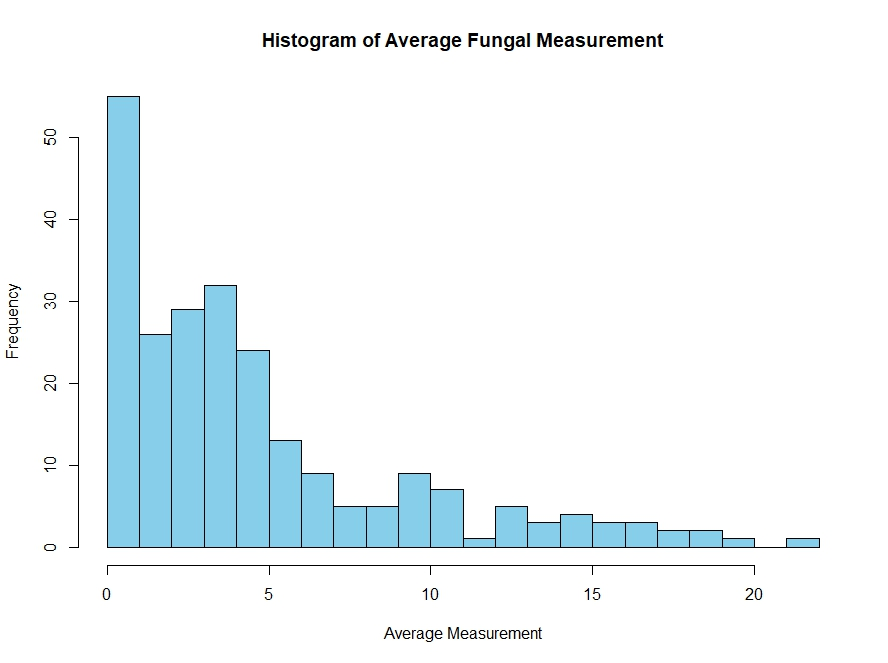
\includegraphics{Fig9.jpeg}

}

\caption{Average Radial growth by Treatment}

\end{figure}

\hypertarget{model-structure}{%
\subsection{Model Structure}\label{model-structure}}

\vspace{-1em}

This study used a zero-inflated Gamma model to examine the effects of
species and treatments on the average fungal growth (positive continuous
measurements with an excess of zeros), while also accounting for the
nested structure of dose. This model was fitted using the
\texttt{glmmTMB} package in R. - The nonzero part (positive fungal
growth) was modelled using a Gamma distribution - The zero-inflated part
which models the probability of an observation being structurally zero
was modelled using a logistic regression. The gamma component consists
of the main effect of species and treatment, interaction between species
and treatment and Random effects for dose nested within treatment. The
zero-inflated component includes only the intercept, assuming a constant
probability of excess zeros across groups. \begin{equation}
Y_{ijkl} \sim \text{Zero inflated Gamma} (\pi_{ijkl}, \alpha, \beta), \text{where}
\end{equation}

\begin{itemize}
\tightlist
\item
  \(Log(E[Y_{ijkl}|Y_{ijkl} > 0]) = \mu + Species_i + Treatment_j + (Species \times Treatment)_{ij} + (1|Dose:Treatment) + (1|Species:Dose:Treatment)\)
\item
  \(Logit(\pi_{ijkl}) = \beta_0\)
\item
  \(\epsilon_{ijkl} \sim Gamma(\alpha, \beta)\)
\end{itemize}

Where:

\begin{itemize}
\tightlist
\item
  \(Y_{ijkl}\) is the average measurement for the \(i\)th species,
  \(j\)th fungicide treatment, \(k\)th dose and \(l\)th dish
\item
  \(\mu\) is the baseline log mean fungal growth
\item
  \(\epsilon_{ijkl}\) is the overall error term
\item
  \(\beta_0\) is the intercept for the zero-inflation model
\end{itemize}

\hypertarget{exploratory-analysis}{%
\subsection{Exploratory Analysis}\label{exploratory-analysis}}

\vspace{-1em}

The individual measurement by treatments plot (Appendix) shows the
distribution of fungal growth across different treatments. Since fungus
spreads out like a circle as it grows, four measurements were taken:
from the center to the top (measurement 1), center to the right
(measurement 2), center to bottom (measurement 3), and center to the
left (measurement 4). This figure shows that the mean growth across the
various measurements was similar across directions, thus we took the
average of the four values for each experimental unit. Figure 2 shows
the average fungal growth across different treatments. Quadris 1 active
ingredient has the highest average fungal growth followed by Endura 1
active ingredient, Topguard EQ 2 active ingredient, and Topguard 1
active ingredient.

\begin{figure}

{\centering 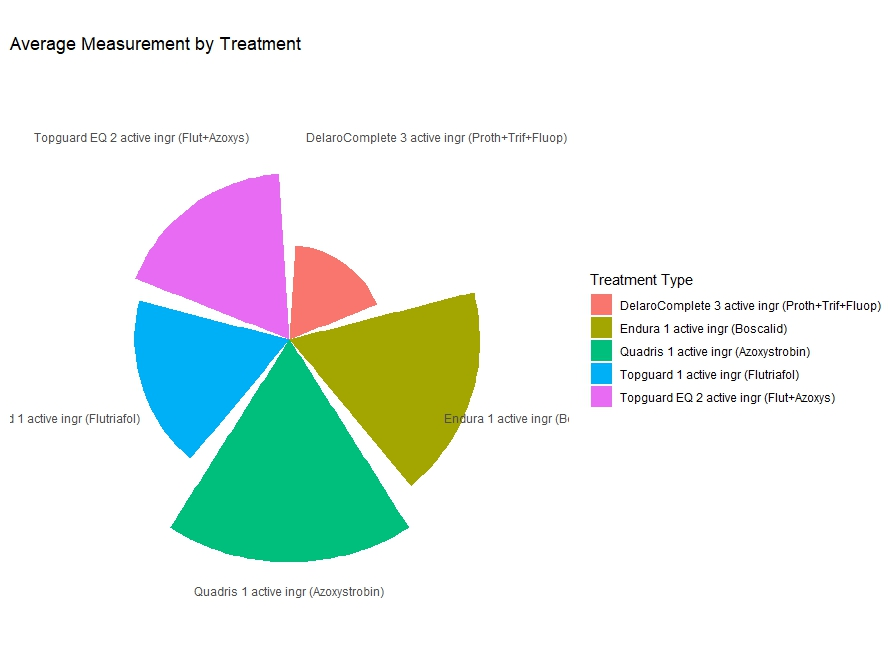
\includegraphics{Fig3.jpeg}

}

\caption{Average Radial growth by Treatment}

\end{figure}

As also observed in the average measurements by treatment plot
(appendix), Quadris 1 active ingredient (Azoxystrobin) showed the
highest median fungal growth and the greatest variability, suggesting
that this treatment was less effective in fungal control compared to the
other treatments. Endura 1 active ingredient (Boscalid) had the next
highest median growth but exhibited slightly less variability. Topguard
1 active ingredient (Flutriafol), Topguard EQ 2 active ingredients
(Flutriafol + Azoxystrobin), and DelaroComplete 3 active ingredients
(Prothioconazole + Trifloxystrobin + Fluopyram) had lower median fungal
growth, which suggests better overall control of fungal spread.

Figure 3 shows the average fungal growth across species. Fusarium
oxysporum grows the highest, followed by Rhizoctonia solani, Fusarium
solani, and Diaporthe longicolla. Figure 6 confirms that Fusarium
oxysporum has the highest growth under the experimental conditions,
while Diaporthe longicolla has the least. Also, the individual
measurement by treatments plot (Appendix) shows the distribution of
fungal growth across different species. As observed in the average
measurements by treatment plot (appendix), the mean growth across the
various measurements was similar across directions.

\begin{figure}

{\centering 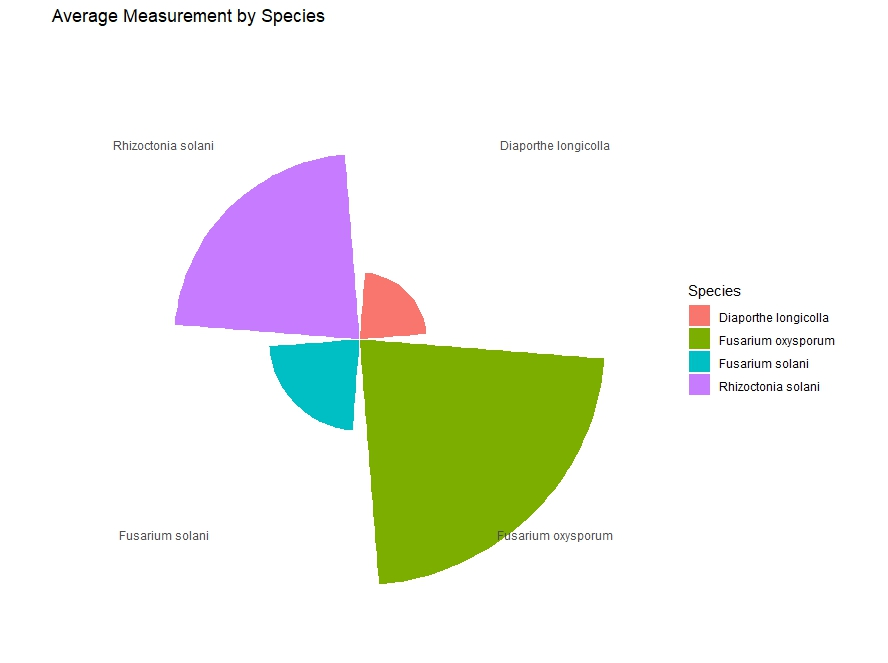
\includegraphics[width=0.5\textwidth,height=\textheight]{Fig4.jpeg}

}

\caption{Average Radial growth by Species}

\end{figure}

Figure 4 shows the distribution of average fungal growth measurements
across different fungicide dose levels, split by fungal species. For
Diaporthe longicolla, the following doses: 6.292, 5.7975, 4.9128,
0.6292, 0.57975, 0.49128, 0.06292, and 0.057975, resulted in complete
inhibition of fungal growth (growth = 0). For Fusarium solani, the doses
of 6.292, 0.6292, and 0.06292 completely inhibited fungal development.
However, Fusarium oxysporum showed resistance to fungicide treatments
across all dose levels. Similar resistance was observed for Rhizoctonia
solani.

\begin{figure}

{\centering 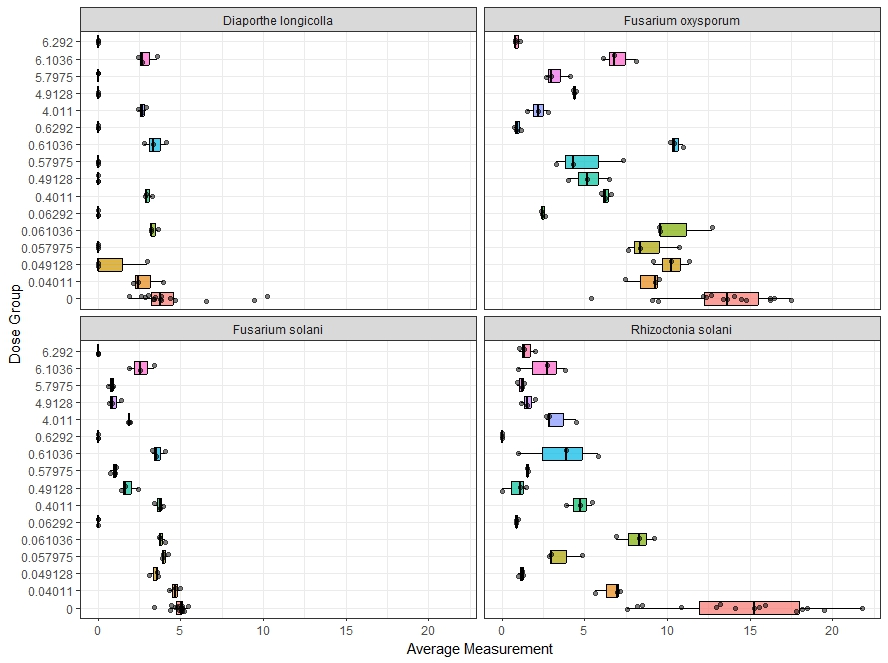
\includegraphics[width=0.5\textwidth,height=\textheight]{Fig7.jpeg}

}

\caption{Fungal Growth by Dose and Species}

\end{figure}

Figure 5 shows the distribution of average fungal growth across
different fungicide dose levels, split by fungicide treatment. This plot
highlights the nested structure of dose within treatment. Across all
treatments, fungal growth decreased with increasing fungicide dose
levels.
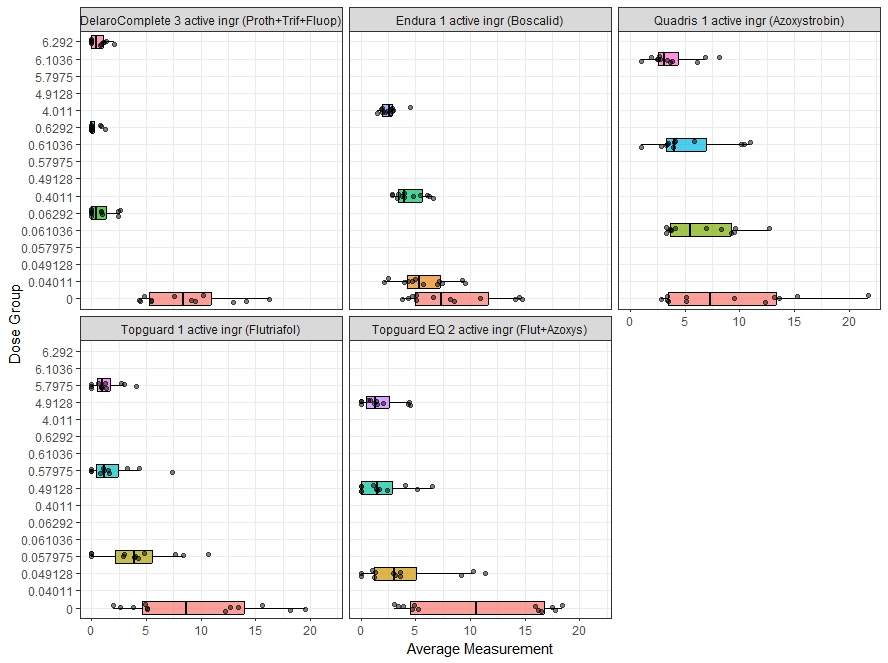
\includegraphics[width=0.5\textwidth,height=\textheight]{Fig8.jpeg}

\hypertarget{advanced-analysis}{%
\section{Advanced Analysis}\label{advanced-analysis}}

\vspace{-1em}

The major goal of performing this experiment is to determine the
effectiveness of fungicides against resistant pathogens.

\hypertarget{random-effect-structure}{%
\subsection{Random Effect Structure:}\label{random-effect-structure}}

\vspace{-1em}

This part of the result shows the nested structure variability in both
the conditional and the zero-inflated model.

Conditional Model Variance Components: These results show the
variability in the pathogen growth for dose nested in treatment and for
species crossed with treatment nested within dose. The variation in
pathogen growth due to the random effect of dose nested within
treatments is 0.3823, while the variation due to the random effect of
species crossed with treatments nested within dose is 0.1007.

\begin{figure}

{\centering 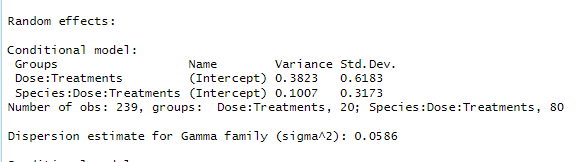
\includegraphics[width=0.5\textwidth,height=\textheight]{Fig10.png}

}

\caption{Radial growth by Species}

\end{figure}

\hypertarget{fixed-effect-structure}{%
\subsection{Fixed Effect Structure}\label{fixed-effect-structure}}

\vspace{-1em}

The ANOVA table shows the effect of species, treatments, and their
interaction for the gamma regression section of the zero-inflated model.
The results indicate a marginally significant interaction between
species and treatment (p \textgreater{} 0.05). We investigated further
to determine which treatment and species combinations differ in growth.
Table 3 shows the interaction between fungal species and different
treatments with respect to their average growth. The results revealed a
statistically significant interaction between Fusarium oxysporum species
and Azoxystrobin treatments (p = 0.0115).

\begin{figure}

{\centering 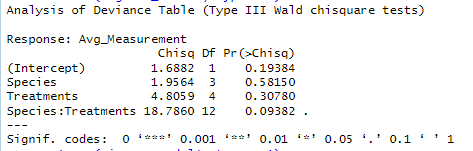
\includegraphics[width=0.5\textwidth,height=\textheight]{Fig11.png}

}

\caption{ANOVA for Fixed Effects}

\end{figure}

\begin{table*}[ht]
\centering
\caption{Interaction between Species and Treatments on Average Growth}
\renewcommand{\arraystretch}{1.2}
\begin{tabular}{|l|l|c|c|c|c|c|c|}
\hline
\rowcolor{gray!15} \textbf{Species} & \textbf{Treatments} & \textbf{df} & \textbf{Avg Growth} & \textbf{SE} & \textbf{LCL} & \textbf{UCL} & \textbf{p} \\
\hline
Diaporthe longicolla & \textit{(Proth+Trif+Fluop)} & 3 & 1.96 & 1.01 & 0.711 & 5.38 & 0.4564 \\
Fusarium oxysporum & \textit{(Proth+Trif+Fluop)} & 3 & 2.2 & 1.0 & 0.614 & 4.081 & 0.3657 \\
Fusarium solani & \textit{(Proth+Trif+Fluop)} & 3 & 1.2 & 0.618 & 0.435 & 3.29 & 0.8737 \\
Rhizoctonia solani & \textit{(Proth+Trif+Fluop)} & 3 & 2.05 & 0.778 & 0.975 & 4.31 & 0.3553 \\
\hline
Diaporthe longicolla & \textit{(Boscalid)} & 1 & 3.27 & 1.1 & 1.651 & 6.5 & 0.9614 \\
Fusarium oxysporum & \textit{(Boscalid)} & 1 & 6.52 & 1.31 & 3.255 & 10.65 & 0.1217 \\
Fusarium solani & \textit{(Boscalid)} & 1 & 5.63 & 1.3 & 2.85 & 10.2 & 0.1703 \\
Rhizoctonia solani & \textit{(Boscalid)} & 1 & 5.61 & 1.19 & 2.874 & 11.27 & 0.2824 \\
\hline
Diaporthe longicolla & \textit{(Azoxystrobin)} & 1 & 3.27 & 1.1 & 1.631 & 6.55 & 0.9614 \\
\rowcolor{yellow!30} Fusarium oxysporum & \textit{(Azoxystrobin)} & 1 & 9.9 & 3.51 & 4.941 & 19.83 & 0.0115 \\
Fusarium solani & \textit{(Azoxystrobin)} & 1 & 3.61 & 1.28 & 1.803 & 7.24 & 0.8737 \\
Rhizoctonia solani & \textit{(Azoxystrobin)} & 1 & 5.99 & 2.2 & 1.184 & 11.99 & 0.1632 \\
\hline
Diaporthe longicolla & \textit{(Flutriafol)} & 1 & 1.05 & 0.52 & 0.399 & 2.77 & 0.5177 \\
Fusarium oxysporum & \textit{(Flutriafol)} & 1 & 6.61 & 2.34 & 2.3 & 13.25 & 0.0894 \\
Fusarium solani & \textit{(Flutriafol)} & 1 & 3.9 & 0.77 & 2.03 & 6.4 & 0.3336 \\
Rhizoctonia solani & \textit{(Flutriafol)} & 1 & 1.92 & 0.646 & 0.905 & 4.04 & 0.2261 \\
\hline
Diaporthe longicolla & \textit{(Flut+Azoxys)} & 2 & 1.89 & 0.785 & 0.835 & 4.27 & 0.3336 \\
Fusarium oxysporum & \textit{(Flut+Azoxys)} & 2 & 2.87 & 0.84 & 1.184 & 4.75 & 0.0913 \\
Fusarium solani & \textit{(Flut+Azoxys)} & 2 & 3.01 & 0.87 & 1.055 & 6.05 & 0.1187 \\
Rhizoctonia solani & \textit{(Flut+Azoxys)} & 2 & 2.6 & 0.926 & 1.298 & 5.23 & 0.6934 \\
\hline
\end{tabular}
\end{table*}

Table 4 shows the significant pairwise comparisons between species and
treatment combinations. Some key findings include:

\begin{itemize}
\tightlist
\item
  Diaporthe longicolla showed 0.33 times lower average growth compared
  to Fusarium oxysporum under Azoxystrobin treatment
\item
  Fusarium oxysporum showed 2.741 times higher average growth compared
  to Fusarium solani under Azoxystrobin treatment
\item
  Fusarium oxysporum under Azoxystrobin treatment showed 9.412 times
  higher average growth compared to Diaporthe longicolla under
  Flutriafol treatment
\item
  Diaporthe longicolla growth was 0.159 times lower than Fusarium
  oxysporum growth under Flutriafol treatment
\item
  Fusarium oxysporum growth was 3.26 times greater than Fusarium solani
  growth when treated with Flutriafol
\end{itemize}

\vspace{0.1cm}

\begin{table*}[ht]
\centering
\caption{Pairwise Differences in Fungal Growth Under Different Treatments}
\renewcommand{\arraystretch}{1.2}
\begin{tabular}{|p{8cm}|c|c|c|c|c|}
\hline
\rowcolor{gray!15} \textbf{Pairwise Comparison} & \textbf{Ratio} & \textbf{SE} & \textbf{LCL} & \textbf{UCL} & \textbf{p-value} \\
\hline
Diaporthe longicolla (Azoxystrobin) / Fusarium oxysporum (Azoxystrobin) & 0.33 & 0.081 & 0.1384 & 0.787 & 0.0011 \\
Fusarium oxysporum (Azoxystrobin) / Fusarium solani (Azoxystrobin) & 2.741 & 0.672 & 1.1489 & 6.537 & 0.0063 \\
Fusarium oxysporum (Azoxystrobin) / Diaporthe longicolla (Flutriafol) & 9.412 & 5.73 & 1.0886 & 81.381 & 0.0313 \\
Diaporthe longicolla (Flutriafol) / Fusarium oxysporum (Flutriafol) & 0.159 & 0.0674 & 0.0354 & 0.714 & 0.0024 \\
Fusarium oxysporum (Flutriafol) / Fusarium solani (Flutriafol) & 3.26 & 0.8 & 1.3664 & 7.776 & 0.0003 \\
Diaporthe longicolla (Flut+Azoxys) / Fusarium oxysporum (Flut+Azoxys) & 0.236 & 0.0773 & 0.0736 & 0.754 & 0.0018 \\
Fusarium oxysporum (Flut+Azoxys) / Fusarium solani (Flut+Azoxys) & 3.378 & 0.829 & 1.416 & 8.058 & 0.0001 \\
Fusarium oxysporum (Flut+Azoxys) / Rhizoctonia solani (Flut+Azoxys) & 3.075 & 0.759 & 1.2826 & 7.374 & 0.0009 \\
\hline
\end{tabular}
\end{table*}

Table 5 shows the Best Linear Unbiased Predictor (BLUP) for the random
factor (dose nested within treatment). The BLUP result describes the
effect of each level of the nested structure on average fungal growth.
The value and sign describe the size and direction of the effect
respectively. The result from the BLUP output below shows that the
highest predicted fungal growth per each of the treatment was observed
when dose was equal to zero. At dose = 0, the treatment DelaroComplete 3
active ingr (Proth+Trif+Fluop) has the highest predicted fungal growth
(BLUP = 1.41), followed by Topguard 1 active ingr (Flutriafol) (BLUP =
0.98), Topguard EQ 2 active ingr (Flut+Azoxys) (BLUP = 0.92), Endura 1
active ingr (Boscalid) (BLUP = 0.46), and Quadris 1 active ingr
(Azoxystrobin) (BLUP = 0.33). For DelaroComplete 3 active ingr
(Proth+Trif+Fluop) treatment, increasing the dose showed a deceasing
trend in the BLUP values, suggesting that higher doses for this
treatment is associated with a reduced fungal growth. For Endura 1
active ingr (Boscalid), the predicted average growth at dose of 0.04011
is 0.13 i.e.~the fungal are predicted to grow by 0.13 for the 0.04011:
Boscalid dose treatment combination, however increasing the dosage to
0.4011 and 4.011 showed a decrease in the average growth of the fungal.
For Quadris 1 active ingr (Azoxystrobin), Topguard 1 active ingr
(Flutriafol), and Topguard EQ 2 active ingr (Flut+Azoxys), we also
observed an increase in the predicted growth of fungus for the second
dose level. However, the third and fourth level showed a decrease in the
predicted growth of fungus.

\begin{figure}

{\centering 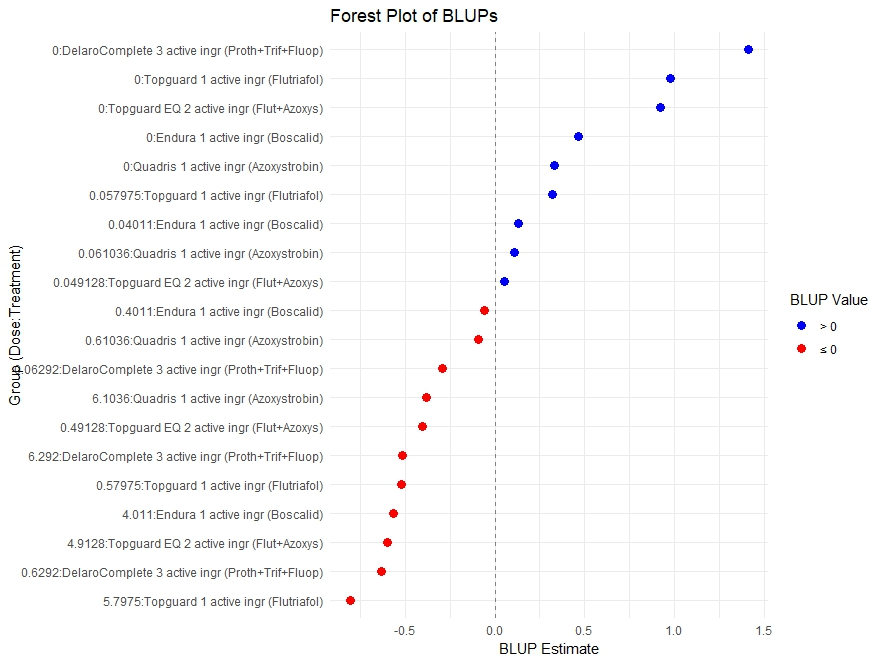
\includegraphics[width=0.5\textwidth,height=\textheight]{Fig18.jpeg}

}

\caption{Fungal Growth by Dose and Treatment}

\end{figure}

A Best Linear Unbiased Prediction (BLUP) was conducted to estimate the
random effects of Species crossed with Dose nested within Treatment, on
fungal growth (Table 6). For Diaporthe Logicolla, increasing growth was
predicted for high dose of Endura 1 active, and Quadris 1 active, low
dose of Topguard EQ2 and medium dose of Quadris 1 active. Stable growth
was predicted for high and medium dose of Delarocomplete, Topguard 1
active, Topguard EQ 1, low and control dose of Delarocomplete and
Toguard 1 active. Other dose treatment combination for this species saw
a decreasing growth. Here, the DelaroComplete (Proth+Trif+Fluop) and
Topguard (Flutriafol) treatment showed little decrease with values close
to zero in BLUP estimates for dose 0 while for other dose, fungus growth
neither increase nor decrease. This suggests that fungal growth under
this treatment remained relatively stable when the dose was increased.
Endura (Boscalid) showed the highest positive BLUP at dose 4.011 (BLUP =
0.298), indicating increased fungal growth at this dose compared to
lower concentrations. However, at lower doses (0.00, 0.04011 and
0.4011), the BLUP estimates were negative, suggesting a decrease in
fungal growth. Quadris (Azoxystrobin) demonstrated negative BLUP
estimates at lower doses (BLUP = -0.282 at dose 0 and -0.063 at dose
0.061) but increased at higher doses (BLUP = 0.12 and 0.22 at 0.61036
and 6.1036 respectively). For Topguard EQ (Flut+Azoxys), the prediction
showed that fungal growth reduced at dose 0, predicted increase in
growth by 0.265 at dose 0.049128 while at dose 0.49128 and 4.9128, there
fungus growth neither increase nor decrease.

For Fusarium oxysporum, increasing growth was predicted for high dose of
Topguard 1 active, Quadris 1 active, Topguard EQ 2, control dose for
Endura 1 active and Delarocomplete, medium dose for Topguard 1 active,
Quadris 1 active, Topguard EQ 2 active, low dose for Delarocomplete,
Topguard EQ 2 active, andEndura 1 active. Other dose treatment
combination for this species saw a decreasing growth. For Fusarium
oxysporum species treated with DelaroComplete 3 active ingr
(Proth+Trif+Fluop) and Quadris 1 active ingr (Azoxystrobin), the Best
Linear Unbiased Prediction result showed an increase in fungus growth
for the first two dose while the fungus growth reduced for the other
dose. For Fusarium oxysporum species treated with Endura 1 active ingr
(Boscalid), the Best Linear Unbiased Prediction result showed an
increase in fungus growth for the first three dose (0.0, 0.04011, and
0.4011) while it predicted a reduction in the growth of fungus for dose
4.011. For Fusarium oxysporum species treated Topguard 1 active ingr
(Flutriafol), BLUP predicted a decrease in growth for dose level 0 and
0.057975 while the other two level is predicted to increase growth in
this specie. For Fusarium oxysporum species treated with Topguard EQ 2
active ingr (Flut+Azoxys), the Best Linear Unbiased Prediction result
showed an increase in fungus growth for dose 0.049128 and 4.9128 while
the other two dose were predicted to reduce growth of fungus.

For Fusarium Solani, increasing growth was predicted for high and medium
dose of Quadris 1 active, medium dose for Endura 1 active, and Topguard
EQ 2, low dose for Topguard 1 active, Topguard Eq 2 active, and Endura 1
active. Stable growth was predicted for high, medium, lowand control
dose of Delarocomplete. Other dose treatment combination for this
species saw a decreasing growth. For Fusarium solani species treated
with DelaroComplete 3 active ingr (Proth+Trif+Fluop), dose 0 showed a
reduction in growth while the other dose level showed a zero growth. For
Fusarium solani species treated with Endura 1 active ingr (Boscalid),
dose 0 and 4.011 showed a reduction in growth while BLUP predicted an
increase in growth for dose 0.04011, and 0.4011. For Fusarium solani
species treated with Topguard 1 active ingr (Flutriafol), BLUP predicted
a reduction in growth at dose 0, 0.57975, and 5.7975 while growth was
predicted to increase at dose level 0.057975. For Fusarium solani
species treated with Topguard EQ 2 active ingr (Flut+Azoxys), dose 0 and
4.9128 showed a reduction in growth while BLUP predicted an increase in
growth for dose 0.049128, and 0.49128.

For Rhizoctonia solani, increasing growth was predicted for control dose
of Topguard EQ 2, Topguard 1 active, Quadris 1 active , Delarocomplete,
and Endura 1 active, low dose of Quadris 1 active and Endura 1 active,
high dose of Delarocomplete, Topguard EQ 2, and Endura 1 active. Stable
growth was predicted for medium Delarocomplete. Other dose treatment
combination for this species saw a decreasing growth. For Rhizoctonia
solani species treated with DelaroComplete 3 active ingr
(Proth+Trif+Fluop) , BLUP showed that dose 0 and 6.292 increased the
fungus growth, dose 0.06292 reduced the fungus growth while dose 0.6292
neither increased nor decrease the growth of fungus. With Endura 1
active ingr (Boscalid) treatment, dose 0.4011 was predicted to reduce
the growth of fungus while the other dose level increased fungus growth.
For Quadris 1 active ingr (Azoxystrobin) treatment, dose 0 and 0.061036
increased fungus growth while the other two dose was predicted to reduce
dose. For Topguard 1 active ingr (Flutriafol), dose 0 and 5.7975 was
predicted to increase fungus growth, while other dose level decreased
the growth of fungus. With Topguard EQ 2 active ingr (Flut+Azoxys), dose
0 and 4.9128 increased the growth of fungus while dose 0.049128 and
0.49128 was predicted to reduce their growth.

\begin{figure}

{\centering 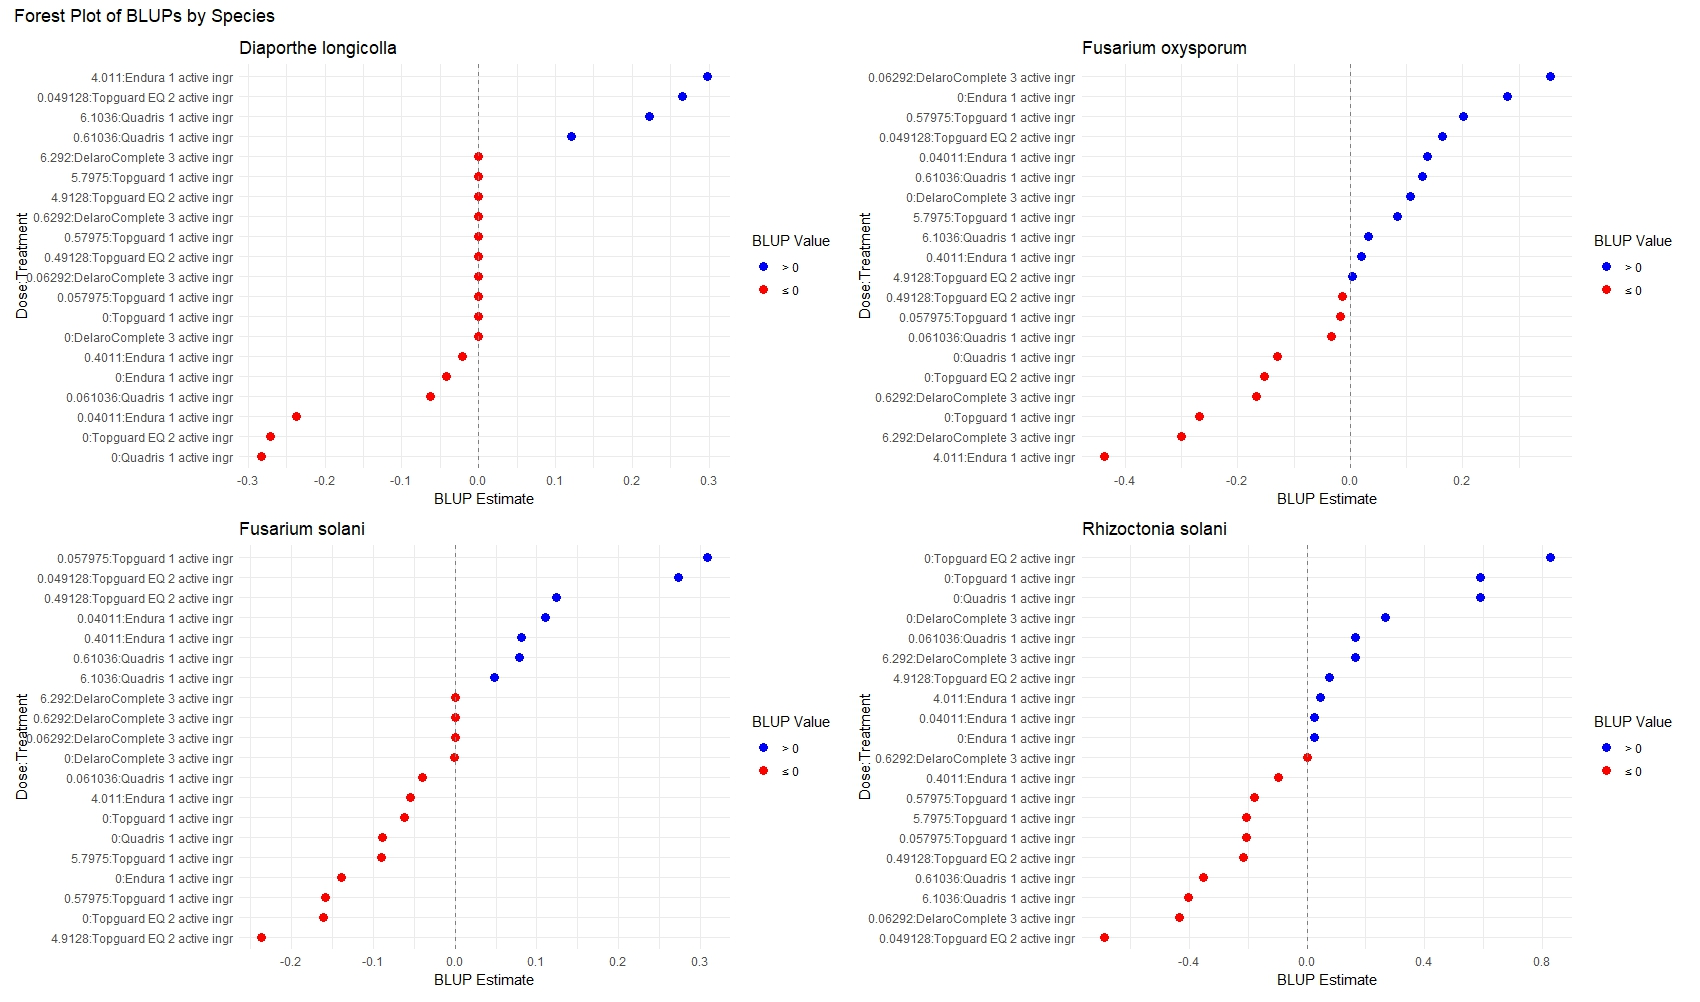
\includegraphics[width=0.5\textwidth,height=\textheight]{Fig21.jpeg}

}

\caption{Fungal Growth by Dose and Treatment}

\end{figure}

\hypertarget{conclusion}{%
\section{Conclusion}\label{conclusion}}

\vspace{-1em}

F. oxysporum differed significantly in growth response compared to
species: F. solani, D. longicolla, R. solani) under the following
treatment Quadris 1 active (Azoxystrobin), Topguard 1 active
(Flutriafol), and Topguard EQ 2 active (Flut+Azoxys). At control dose,
delarocomplete treatment has the highest growth, followed by Topguard 1
active, Topguard EQ 2 active, Endura 1 active, Quadris 1 active.
Topguard 1 active, Topguard EQ 2 active, Endura 1 active, Quadris 1
active continued to grow at low dose but delarocomplete decreased in
growth. For species crossed with dose nested in treatments, responses
varied by species and fungicide, indicating strong species-specific
interaction patterns. Notable differences for F. oxysporum, which showed
variable trends depending on treatment and dose. Overall, effective
fungal control depends on both selecting the right treatment and
optimizing dose for the specific species involved.

\hypertarget{references}{%
\section{References}\label{references}}

\hypertarget{refs}{}
\begin{CSLReferences}{1}{0}
\leavevmode\vadjust pre{\hypertarget{ref-Allen2023}{}}%
Allen, T. et al. 2023. {``Soybean Disease Loss Estimates from the United
States and Ontario, Canada --- 2022.''}
\url{https://doi.org/10.31274/cpn-20230421-1}.

\leavevmode\vadjust pre{\hypertarget{ref-Altalb_2009}{}}%
Altalb, Ahmed Awad. 2009. {``EFFICACY OF CHEMICAL AND BIOLOGICAL
TREATMENTS FOR CONTROLLING SOIL-BORNE PATHOGENS OF SOYBEAN.''}
\emph{Arab Universities Journal of Agricultural Sciences} 17 (1):
163--73. \url{https://doi.org/10.21608/ajs.2009.14844}.

\leavevmode\vadjust pre{\hypertarget{ref-Cropwatch}{}}%
CropWatch, University of Nebraska-Lincoln. n.d. {``Soybean Disease
Management.''} \url{https://cropwatch.unl.edu/plant-disease/soybean/}.

\leavevmode\vadjust pre{\hypertarget{ref-farmjournal2025}{}}%
Farm Journal. 2025. {``Soybean Blight: How to Identify Pythium,
Phytophthora, Fusarium, and Rhizoctonia.''}
\url{https://www.agweb.com/news/crops/how-identify-soybean-blight}.

\leavevmode\vadjust pre{\hypertarget{ref-Gianessi_Reigner_2007}{}}%
Gianessi, Leonard P., and Nathan P. Reigner. 2007. {``The Value of
Herbicides in u.s. Crop Production.''} \emph{Weed Technology} 21 (2):
559--66. \url{https://doi.org/10.1614/WT-06-130.1}.

\leavevmode\vadjust pre{\hypertarget{ref-Mills2013}{}}%
Mills, E. D. 2013. {``Adjusting for Covariates in Zero-Inflated Gamma
and Zero-Inflated Log-Normal Models.''} PhD thesis, University of Iowa.

\leavevmode\vadjust pre{\hypertarget{ref-S_Navi2016}{}}%
Navi, S., and A. Rajasab. 2016. {``In Vitro Evaluation of Commercial
Fungicides Against Major Soil-Borne Pathogens of Soybean.''}
\emph{Journal of Plant Pathology \& Microbiology} 7 (3).
\url{https://doi.org/10.4172/2157-7471.1000340}.

\leavevmode\vadjust pre{\hypertarget{ref-sang_2023}{}}%
Sang, X. Yuan, Y. Liu, and Y. Wang. 2023. {``Genome-Wide Association
Study on Resistance of Cultivated Soybean to Fusarium Oxysporum Root Rot
in Northeast China,''} December. \url{https://doi.org/10.1101/637652}.

\leavevmode\vadjust pre{\hypertarget{ref-USA2025}{}}%
USDA. 2025. {``Production - Soybeans.''}
\url{https://www.fas.usda.gov/data/production/commodity/2222000}.

\leavevmode\vadjust pre{\hypertarget{ref-Wei_2019}{}}%
Wei, Xue-Xin, Ding Zhou, Andres Grosmark, Zaki Ajabi, Fraser Sparks,
Pengcheng Zhou, Mark Brandon, Attila Losonczy, and Liam Paninski. 2019.
{``A Zero-Inflated Gamma Model for Post-Deconvolved Calcium Imaging
Traces,''} May. \url{https://doi.org/10.1101/637652}.

\end{CSLReferences}

\clearpage
\nocite{*}
\twocolumn[\section*{Appendix I}]

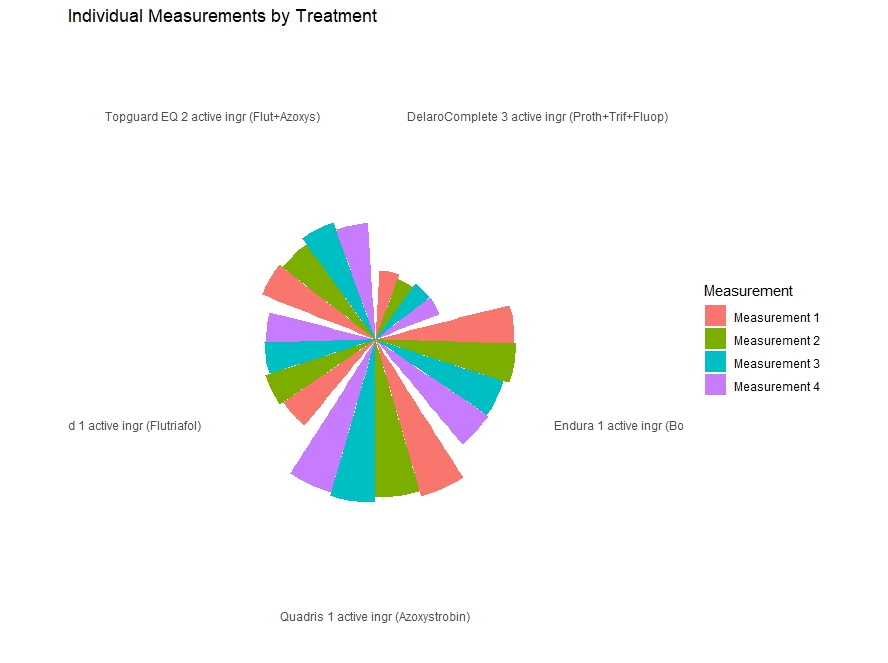
\includegraphics[width=0.45\textwidth,height=\textheight]{Fig1.jpeg}
\vspace{0.1cm}
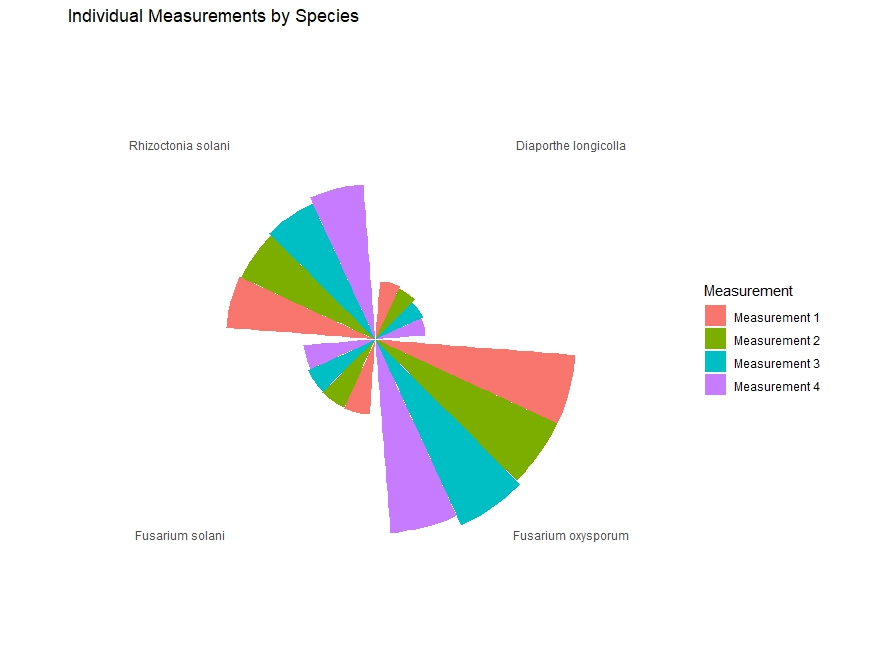
\includegraphics[width=0.45\textwidth,height=\textheight]{Fig2.jpeg}
\vspace{0.1cm}
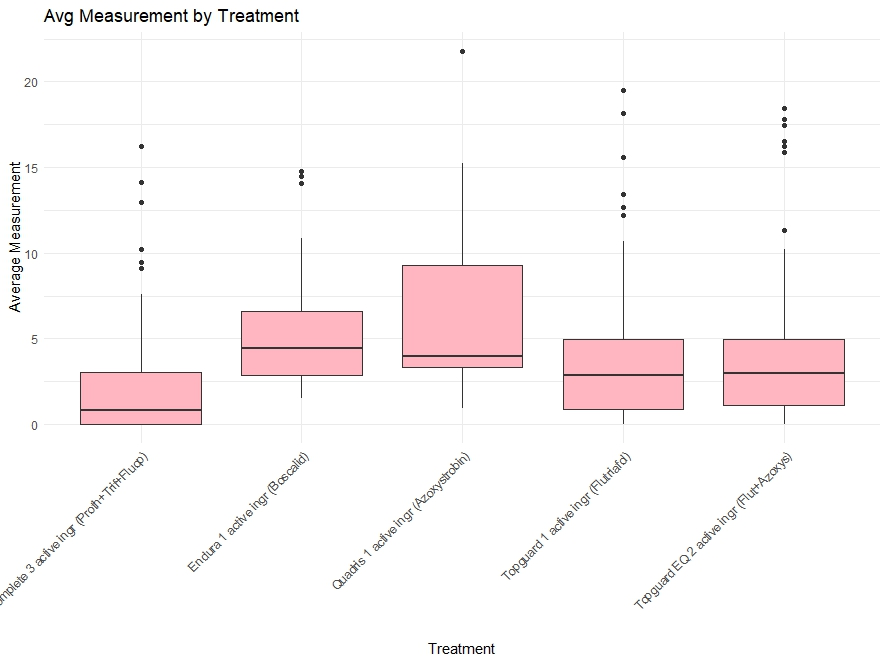
\includegraphics[width=0.45\textwidth,height=\textheight]{Fig5.jpeg}
\vspace{0.1cm}
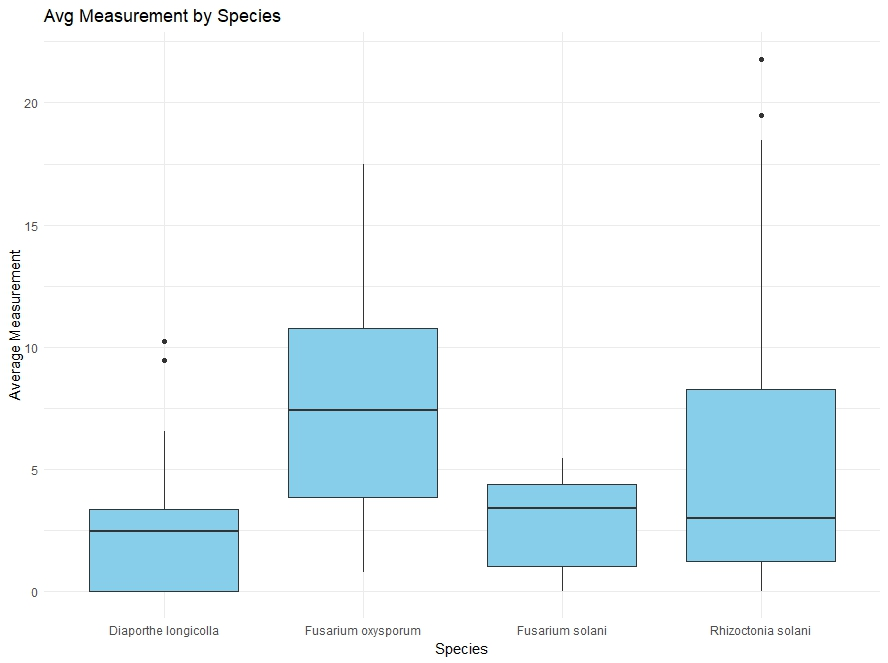
\includegraphics[width=0.45\textwidth,height=\textheight]{Fig6.jpeg}
\vspace{0.1cm}

\begin{table}[ht]
\centering
\small
\caption{Best Linear Unbiased Prediction for Dose nested within Treatment}
\renewcommand{\arraystretch}{1.2}
\begin{tabular}{|p{7.0cm}|r|}
\hline
\textbf{Dose:Treatment} & \textbf{BLUP} \\
\hline
0:DelaroComplete 3 active \textit{(Proth+Trif+Fluop)} & 1.4118 \\
0.06292:DelaroComplete 3 active \textit{(Proth+Trif+Fluop)} & -0.2938 \\
0.6292:DelaroComplete 3 active \textit{(Proth+Trif+Fluop)} & -0.6315 \\
6.292:DelaroComplete 3 active \textit{(Proth+Trif+Fluop)} & -0.5171 \\
0:Endura 1 active \textit{(Boscalid)} & 0.4644 \\
0.04011:Endura 1 active \textit{(Boscalid)} & 0.1312 \\
0.4011:Endura 1 active \textit{(Boscalid)} & -0.0614 \\
4.011:Endura 1 active \textit{(Boscalid)} & -0.5659 \\
0:Quadris 1 active \textit{(Azoxystrobin)} & 0.3327 \\
0.061036:Quadris 1 active \textit{(Azoxystrobin)} & 0.1095 \\
0.61036:Quadris 1 active \textit{(Azoxystrobin)} & -0.0933 \\
6.1036:Quadris 1 active \textit{(Azoxystrobin)} & -0.3806 \\
0:Topguard 1 active \textit{(Flutriafol)} & 0.9781 \\
0.057975:Topguard 1 active \textit{(Flutriafol)} & 0.3181 \\
0.57975:Topguard 1 active \textit{(Flutriafol)} & -0.5203 \\
5.7975:Topguard 1 active \textit{(Flutriafol)} & -0.8084 \\
0:Topguard EQ 2 active \textit{(Flut+Azoxys)} & 0.9204 \\
0.049128:Topguard EQ 2 active \textit{(Flut+Azoxys)} & 0.0501 \\
0.49128:Topguard EQ 2 active \textit{(Flut+Azoxys)} & -0.4068 \\
4.9128:Topguard EQ 2 active \textit{(Flut+Azoxys)} & -0.5986 \\
\hline
\end{tabular}
\end{table}

\vspace{0.1cm}

\begin{table}[ht]
\centering
\small
\caption{Best Linear Unbiased Prediction for Dose nested within Treatment for Diaporthe longicolla }
\renewcommand{\arraystretch}{1.2}
\begin{tabular}{|p{6.4cm}|r|}
\hline
\textbf{Dose:Treatment} & \textbf{BLUP} \\
\hline
0:DelaroComplete 3 active \textit{(Proth+Trif+Fluop)} & -0.000616511 \\
0.06292:DelaroComplete 3 active \textit{(Proth+Trif+Fluop)} & 0 \\
0.6292:DelaroComplete 3 active \textit{(Proth+Trif+Fluop)} & 0 \\
6.292:DelaroComplete 3 active \textit{(Proth+Trif+Fluop)} & 0 \\
0:Endura 1 active \textit{(Boscalid)} & -0.041562794 \\
0.04011:Endura 1 active \textit{(Boscalid)} & -0.237818396 \\
0.4011:Endura 1 active \textit{(Boscalid)} & -0.021039568 \\
4.011:Endura 1 active \textit{(Boscalid)} & 0.298317876 \\
0:Quadris 1 active \textit{(Azoxystrobin)} & -0.282390186 \\
0.061036:Quadris 1 active \textit{(Azoxystrobin)} & -0.062961318 \\
0.61036:Quadris 1 active \textit{(Azoxystrobin)} & 0.121451677 \\
6.1036:Quadris 1 active \textit{(Azoxystrobin)} & 0.221821793 \\
0:Topguard 1 active \textit{(Flutriafol)} & -0.000574947 \\
0.057975:Topguard 1 active \textit{(Flutriafol)} & 0 \\
0.57975:Topguard 1 active \textit{(Flutriafol)} & 0 \\
5.7975:Topguard 1 active \textit{(Flutriafol)} & 0 \\
0:Topguard EQ 2 active \textit{(Flut+Azoxys)} & -0.271722003 \\
0.049128:Topguard EQ 2 active \textit{(Flut+Azoxys)} & 0.265117379 \\
0.49128:Topguard EQ 2 active \textit{(Flut+Azoxys)} & 0 \\
4.9128:Topguard EQ 2 active \textit{(Flut+Azoxys)} & 0 \\
\hline
\end{tabular}
\end{table}

\vspace{0.1cm}

\begin{table}[ht]
\centering
\small
\caption{Best Linear Unbiased Prediction for Dose nested within Treatment for Fusarium oxysporum }
\renewcommand{\arraystretch}{1.2}
\begin{tabular}{|p{6.4cm}|r|}
\hline
\textbf{Dose:Treatment} & \textbf{BLUP} \\
\hline
0:DelaroComplete 3 active \textit{(Proth+Trif+Fluop)} & 0.106100059 \\
0.06292:DelaroComplete 3 active \textit{(Proth+Trif+Fluop)} & 0.355692318\\
0.6292:DelaroComplete 3 active \textit{(Proth+Trif+Fluop)} & -0.166327429 \\
6.292:DelaroComplete 3 active \textit{(Proth+Trif+Fluop)} & -0.299732171 \\
0:Endura 1 active \textit{(Boscalid)} & 0.278496151 \\
0.04011:Endura 1 active \textit{(Boscalid)} & 0.136230476 \\
0.4011:Endura 1 active \textit{(Boscalid)} & 0.019989513 \\
4.011:Endura 1 active \textit{(Boscalid)} & -0.436805234 \\
0:Quadris 1 active \textit{(Azoxystrobin)} & -0.129392723 \\
0.061036:Quadris 1 active \textit{(Azoxystrobin)} & -0.034205375 \\
0.61036:Quadris 1 active \textit{(Azoxystrobin)} & 0.128827724 \\
6.1036:Quadris 1 active \textit{(Azoxystrobin)} & 0.032736257 \\
0:Topguard 1 active \textit{(Flutriafol)} & -0.268141692 \\
0.057975:Topguard 1 active \textit{(Flutriafol)} & -0.017637166 \\
0.57975:Topguard 1 active \textit{(Flutriafol)} & 0.200686125 \\
5.7975:Topguard 1 active \textit{(Flutriafol)} & 0.083511652 \\
0:Topguard EQ 2 active \textit{(Flut+Azoxys)} & -0.153415918 \\
0.049128:Topguard EQ 2 active \textit{(Flut+Azoxys)} & 0.164391125 \\
0.49128:Topguard EQ 2 active \textit{(Flut+Azoxys)} & -0.014750217 \\
4.9128:Topguard EQ 2 active \textit{(Flut+Azoxys)} & 0.004023557 \\
\hline
\end{tabular}
\end{table}

\vspace{0.1cm}

\begin{table}[ht]
\centering
\small
\caption{Best Linear Unbiased Prediction for Dose nested within Treatment for Fusarium solani }
\renewcommand{\arraystretch}{1.2}
\begin{tabular}{|p{6.4cm}|r|}
\hline
\textbf{Dose:Treatment} & \textbf{BLUP} \\
\hline
0:DelaroComplete 3 active \textit{(Proth+Trif+Fluop)} & -0.000625527 \\
0.06292:DelaroComplete 3 active \textit{(Proth+Trif+Fluop)} & 0\\
0.6292:DelaroComplete 3 active \textit{(Proth+Trif+Fluop)} & 0 \\
6.292:DelaroComplete 3 active \textit{(Proth+Trif+Fluop)} & 0 \\
0:Endura 1 active \textit{(Boscalid)} & -0.13874485 \\
0.04011:Endura 1 active \textit{(Boscalid)} & 0.110523464 \\
0.4011:Endura 1 active \textit{(Boscalid)} & 0.080927519 \\
4.011:Endura 1 active \textit{(Boscalid)} & -0.05479903 \\
0:Quadris 1 active \textit{(Azoxystrobin)} & -0.088966249 \\
0.061036:Quadris 1 active \textit{(Azoxystrobin)} & -0.04005418 \\
0.61036:Quadris 1 active \textit{(Azoxystrobin)} & 0.078676058 \\
6.1036:Quadris 1 active \textit{(Azoxystrobin)} & 0.048275351 \\
0:Topguard 1 active \textit{(Flutriafol)} & -0.062226152\\
0.057975:Topguard 1 active \textit{(Flutriafol)} & 0.308842891 \\
0.57975:Topguard 1 active \textit{(Flutriafol)} & -0.158526749 \\
5.7975:Topguard 1 active \textit{(Flutriafol)} & -0.089786457 \\
0:Topguard EQ 2 active \textit{(Flut+Azoxys)} & -0.160570939 \\
0.049128:Topguard EQ 2 active \textit{(Flut+Azoxys)} & 0.272726683 \\
0.49128:Topguard EQ 2 active \textit{(Flut+Azoxys)} & 0.124419505 \\
4.9128:Topguard EQ 2 active \textit{(Flut+Azoxys)} & -0.236335868 \\
\hline
\end{tabular}
\end{table}

\vspace{0.1cm}

\begin{table}[ht]
\centering
\small
\caption{Best Linear Unbiased Prediction for Dose nested within Treatment for Rhizoctonia solani }
\renewcommand{\arraystretch}{1.2}
\begin{tabular}{|p{6.4cm}|r|}
\hline
\textbf{Dose:Treatment} & \textbf{BLUP} \\
\hline
0:DelaroComplete 3 active \textit{(Proth+Trif+Fluop)} & 0.266911298 \\
0.06292:DelaroComplete 3 active \textit{(Proth+Trif+Fluop)} & -0.433046666\\
0.6292:DelaroComplete 3 active \textit{(Proth+Trif+Fluop)} & 0 \\
6.292:DelaroComplete 3 active \textit{(Proth+Trif+Fluop)} & 0.163567614 \\
0:Endura 1 active \textit{(Boscalid)} & 0.02410454 \\
0.04011:Endura 1 active \textit{(Boscalid)} & 0.025606511 \\
0.4011:Endura 1 active \textit{(Boscalid)} & -0.09605766 \\
4.011:Endura 1 active \textit{(Boscalid)} & 0.044278398 \\
0:Quadris 1 active \textit{(Azoxystrobin)} & 0.588356584 \\
0.061036:Quadris 1 active \textit{(Azoxystrobin)} & 0.166050995 \\
0.61036:Quadris 1 active \textit{(Azoxystrobin)} & -0.353527076 \\
6.1036:Quadris 1 active \textit{(Azoxystrobin)} & -0.403055423 \\
0:Topguard 1 active \textit{(Flutriafol)} & 0.588507333\\
0.057975:Topguard 1 active \textit{(Flutriafol)} & -0.20745378 \\
0.57975:Topguard 1 active \textit{(Flutriafol)} & -0.179171739 \\
5.7975:Topguard 1 active \textit{(Flutriafol)} & -0.206618072 \\
0:Topguard EQ 2 active \textit{(Flut+Azoxys)} & 0.828083859\\
0.049128:Topguard EQ 2 active \textit{(Flut+Azoxys)} & -0.689032837 \\
0.49128:Topguard EQ 2 active \textit{(Flut+Azoxys)} & -0.216787688 \\
4.9128:Topguard EQ 2 active \textit{(Flut+Azoxys)} & 0.074685212 \\
\hline
\end{tabular}
\end{table}

\clearpage
\nocite{*}
\onecolumn
\section*{Appendix II}
\scriptsize

\begin{Shaded}
\begin{Highlighting}[]
\FunctionTok{library}\NormalTok{(readr)}
\FunctionTok{library}\NormalTok{(dplyr)}
\FunctionTok{library}\NormalTok{(car)}
\FunctionTok{library}\NormalTok{(lme4)}
\FunctionTok{library}\NormalTok{(glmmTMB)}
\FunctionTok{library}\NormalTok{(tidyr)}
\FunctionTok{library}\NormalTok{(ggplot2)}
\FunctionTok{library}\NormalTok{(stringr)}
\FunctionTok{library}\NormalTok{(forcats)}
\FunctionTok{library}\NormalTok{(tidyr)}
\FunctionTok{library}\NormalTok{(patchwork)}

\CommentTok{\#Data Import}
\NormalTok{Fungicide\_Data }\OtherTok{\textless{}{-}} \FunctionTok{read\_csv}\NormalTok{(}\StringTok{"Fungicide Exp 5 Design.csv"}\NormalTok{)}
\FunctionTok{View}\NormalTok{(Fungicide\_Data)}

\FunctionTok{str}\NormalTok{(Fungicide\_Data)}


\CommentTok{\# Pivot the measurement columns into long format}
\NormalTok{Fungicide\_long }\OtherTok{\textless{}{-}}\NormalTok{ Fungicide\_Data }\SpecialCharTok{\%\textgreater{}\%}
  \FunctionTok{pivot\_longer}\NormalTok{(}\AttributeTok{cols =} \FunctionTok{starts\_with}\NormalTok{(}\StringTok{"Measurement"}\NormalTok{), }
               \AttributeTok{names\_to =} \StringTok{"Measurement\_Number"}\NormalTok{, }
               \AttributeTok{values\_to =} \StringTok{"Measurement\_Value"}\NormalTok{) }\SpecialCharTok{\%\textgreater{}\%}
  \FunctionTok{filter}\NormalTok{(}\SpecialCharTok{!}\FunctionTok{is.na}\NormalTok{(Measurement\_Value))  }\CommentTok{\# Remove missing values if needed}

\CommentTok{\# Quick check}
\FunctionTok{head}\NormalTok{(Fungicide\_long)}


\CommentTok{\# Summarize if needed}
\NormalTok{fungicide\_summary\_long }\OtherTok{\textless{}{-}}\NormalTok{ Fungicide\_long }\SpecialCharTok{\%\textgreater{}\%}
  \FunctionTok{group\_by}\NormalTok{(Treatments, Measurement\_Number) }\SpecialCharTok{\%\textgreater{}\%}
  \FunctionTok{summarise}\NormalTok{(}\AttributeTok{Avg\_Length =} \FunctionTok{mean}\NormalTok{(Measurement\_Value, }\AttributeTok{na.rm =} \ConstantTok{TRUE}\NormalTok{)) }\SpecialCharTok{\%\textgreater{}\%}
  \FunctionTok{ungroup}\NormalTok{()}

\CommentTok{\# Plot}
\FunctionTok{ggplot}\NormalTok{(fungicide\_summary\_long, }\FunctionTok{aes}\NormalTok{(}\AttributeTok{x =}\NormalTok{ Treatments, }\AttributeTok{y =}\NormalTok{ Avg\_Length, }\AttributeTok{fill =}\NormalTok{ Measurement\_Number)) }\SpecialCharTok{+}
  \FunctionTok{geom\_bar}\NormalTok{(}\AttributeTok{stat =} \StringTok{"identity"}\NormalTok{, }\AttributeTok{position =} \StringTok{"dodge"}\NormalTok{) }\SpecialCharTok{+}  \CommentTok{\# You can also try position = "stack"}
  \FunctionTok{coord\_polar}\NormalTok{(}\AttributeTok{start =} \DecValTok{0}\NormalTok{) }\SpecialCharTok{+}
  \FunctionTok{ylim}\NormalTok{(}\DecValTok{0}\NormalTok{, }\FunctionTok{max}\NormalTok{(fungicide\_summary\_long}\SpecialCharTok{$}\NormalTok{Avg\_Length) }\SpecialCharTok{*} \FloatTok{1.5}\NormalTok{) }\SpecialCharTok{+}
  \FunctionTok{theme\_minimal}\NormalTok{() }\SpecialCharTok{+}
  \FunctionTok{theme}\NormalTok{(}
    \AttributeTok{axis.text.y =} \FunctionTok{element\_blank}\NormalTok{(),}
    \AttributeTok{axis.ticks =} \FunctionTok{element\_blank}\NormalTok{(),}
    \AttributeTok{axis.title =} \FunctionTok{element\_blank}\NormalTok{(),}
    \AttributeTok{panel.grid =} \FunctionTok{element\_blank}\NormalTok{(),}
    \AttributeTok{legend.position =} \StringTok{"right"}
\NormalTok{  ) }\SpecialCharTok{+}
  \FunctionTok{labs}\NormalTok{(}\AttributeTok{fill =} \StringTok{"Measurement"}\NormalTok{, }\AttributeTok{title =} \StringTok{"Individual Measurements by Treatment"}\NormalTok{)}

\NormalTok{fungicide\_summary\_long2 }\OtherTok{\textless{}{-}}\NormalTok{ Fungicide\_long }\SpecialCharTok{\%\textgreater{}\%}
  \FunctionTok{group\_by}\NormalTok{(Species, Measurement\_Number) }\SpecialCharTok{\%\textgreater{}\%}
  \FunctionTok{summarise}\NormalTok{(}\AttributeTok{Avg\_Length =} \FunctionTok{mean}\NormalTok{(Measurement\_Value, }\AttributeTok{na.rm =} \ConstantTok{TRUE}\NormalTok{)) }\SpecialCharTok{\%\textgreater{}\%}
  \FunctionTok{ungroup}\NormalTok{()}

\FunctionTok{ggplot}\NormalTok{(fungicide\_summary\_long2, }\FunctionTok{aes}\NormalTok{(}\AttributeTok{x =}\NormalTok{ Species, }\AttributeTok{y =}\NormalTok{ Avg\_Length, }\AttributeTok{fill =}\NormalTok{ Measurement\_Number)) }\SpecialCharTok{+}
  \FunctionTok{geom\_bar}\NormalTok{(}\AttributeTok{stat =} \StringTok{"identity"}\NormalTok{, }\AttributeTok{position =} \StringTok{"dodge"}\NormalTok{) }\SpecialCharTok{+}  \CommentTok{\# You can also try position = "stack"}
  \FunctionTok{coord\_polar}\NormalTok{(}\AttributeTok{start =} \DecValTok{0}\NormalTok{) }\SpecialCharTok{+}
  \FunctionTok{ylim}\NormalTok{(}\DecValTok{0}\NormalTok{, }\FunctionTok{max}\NormalTok{(fungicide\_summary\_long}\SpecialCharTok{$}\NormalTok{Avg\_Length) }\SpecialCharTok{*} \FloatTok{1.5}\NormalTok{) }\SpecialCharTok{+}
  \FunctionTok{theme\_minimal}\NormalTok{() }\SpecialCharTok{+}
  \FunctionTok{theme}\NormalTok{(}
    \AttributeTok{axis.text.y =} \FunctionTok{element\_blank}\NormalTok{(),}
    \AttributeTok{axis.ticks =} \FunctionTok{element\_blank}\NormalTok{(),}
    \AttributeTok{axis.title =} \FunctionTok{element\_blank}\NormalTok{(),}
    \AttributeTok{panel.grid =} \FunctionTok{element\_blank}\NormalTok{(),}
    \AttributeTok{legend.position =} \StringTok{"right"}
\NormalTok{  ) }\SpecialCharTok{+}
  \FunctionTok{labs}\NormalTok{(}\AttributeTok{fill =} \StringTok{"Measurement"}\NormalTok{, }\AttributeTok{title =} \StringTok{"Individual Measurements by Species"}\NormalTok{)}


\NormalTok{Fungicide\_Data}\SpecialCharTok{$}\NormalTok{Avg\_Measurement }\OtherTok{\textless{}{-}} \FunctionTok{rowMeans}\NormalTok{(Fungicide\_Data[,}\FunctionTok{c}\NormalTok{(}\StringTok{"Measurement 1"}\NormalTok{,}\StringTok{"Measurement 2"}\NormalTok{, }\StringTok{"Measurement 3"}\NormalTok{,}\StringTok{"Measurement 4"}\NormalTok{)], }\AttributeTok{na.rm =} \ConstantTok{TRUE}\NormalTok{)}
\FunctionTok{summary}\NormalTok{(Fungicide\_Data}\SpecialCharTok{$}\NormalTok{Avg\_Measurement)}

\NormalTok{Fungicide\_Data[}\FunctionTok{is.na}\NormalTok{(Fungicide\_Data}\SpecialCharTok{$}\NormalTok{Avg\_Measurement),]}
\NormalTok{Fungicide\_Data }\OtherTok{\textless{}{-}}\NormalTok{ Fungicide\_Data[}\SpecialCharTok{!}\FunctionTok{is.na}\NormalTok{(Fungicide\_Data}\SpecialCharTok{$}\NormalTok{Avg\_Measurement), ]}


\CommentTok{\# Remove the four measurement columns}
\NormalTok{Fungicide\_Data }\OtherTok{\textless{}{-}}\NormalTok{ Fungicide\_Data[, }\SpecialCharTok{!}\NormalTok{(}\FunctionTok{names}\NormalTok{(Fungicide\_Data) }\SpecialCharTok{\%in\%} \FunctionTok{c}\NormalTok{(}\StringTok{"Measurement 1"}\NormalTok{, }\StringTok{"Measurement 2"}\NormalTok{, }\StringTok{"Measurement 3"}\NormalTok{, }\StringTok{"Measurement 4"}\NormalTok{,}\StringTok{"Comments"}\NormalTok{,}\StringTok{"Dates"}\NormalTok{))]}
\FunctionTok{str}\NormalTok{(Fungicide\_Data)}


\CommentTok{\# Rename variables}
\NormalTok{Fungicide\_Data }\OtherTok{\textless{}{-}}\NormalTok{ Fungicide\_Data }\SpecialCharTok{\%\textgreater{}\%} \FunctionTok{rename}\NormalTok{(}\AttributeTok{Dose =}\NormalTok{ ...}\DecValTok{10}\NormalTok{)}

\CommentTok{\#Converting to a Factor}
\NormalTok{Fungicide\_Data }\OtherTok{\textless{}{-}}\NormalTok{ Fungicide\_Data }\SpecialCharTok{\%\textgreater{}\%}
  \FunctionTok{mutate}\NormalTok{(}
    \AttributeTok{Species =} \FunctionTok{as.factor}\NormalTok{(Species),}
    \AttributeTok{Isolates =} \FunctionTok{as.factor}\NormalTok{(Isolates),}
    \AttributeTok{Treatments =} \FunctionTok{as.factor}\NormalTok{(Treatments),}
    \AttributeTok{Dilution =} \FunctionTok{as.factor}\NormalTok{(Dilution),}
    \AttributeTok{techRep =} \FunctionTok{as.factor}\NormalTok{(techRep),}
    \AttributeTok{Exp\_Code =} \FunctionTok{as.factor}\NormalTok{(Exp\_Code),}
    \AttributeTok{Dose =} \FunctionTok{as.factor}\NormalTok{(Dose)}
\NormalTok{  )}

\CommentTok{\# Check the structure of the dataset}
\FunctionTok{str}\NormalTok{(Fungicide\_Data)}
\FunctionTok{summary}\NormalTok{(Fungicide\_Data)}

\DocumentationTok{\#\#\#\#\#\#\#\#\#\#\#\#\#\#\#\#\#\#\#\#\#\#\#\#\#\#\#\#\#\#\#\#\#\#\#\#\#\#\#Exploratory Data Analysis\#\#\#\#\#\#\#\#\#\#\#\#\#\#\#\#\#\#\#\#\#\#\#\#\#\#\#\#\#\#\#\#\#\#\#\#\#\#\#\#\#\#\#\#\#\#\#\#\#\#\#\#\#\#\#\#\#}
\FunctionTok{hist}\NormalTok{(Fungicide\_Data}\SpecialCharTok{$}\NormalTok{Avg\_Measurement, }
     \AttributeTok{breaks =} \DecValTok{30}\NormalTok{, }
     \AttributeTok{main =} \StringTok{"Histogram of Average Fungal Measurement"}\NormalTok{,}
     \AttributeTok{xlab =} \StringTok{"Average Measurement"}\NormalTok{,}
     \AttributeTok{col =} \StringTok{"skyblue"}\NormalTok{)}

\FunctionTok{ggplot}\NormalTok{(Fungicide\_Data, }\FunctionTok{aes}\NormalTok{(}\AttributeTok{x =}\NormalTok{ Species, }\AttributeTok{y =}\NormalTok{ Avg\_Measurement)) }\SpecialCharTok{+}
  \FunctionTok{geom\_boxplot}\NormalTok{(}\AttributeTok{fill =} \StringTok{"skyblue"}\NormalTok{) }\SpecialCharTok{+}
  \FunctionTok{theme\_minimal}\NormalTok{() }\SpecialCharTok{+}   \CommentTok{\#white background}
  \FunctionTok{labs}\NormalTok{(}\AttributeTok{title =} \StringTok{"Avg Measurement by Species"}\NormalTok{,}
       \AttributeTok{x =} \StringTok{"Species"}\NormalTok{,}
       \AttributeTok{y =} \StringTok{"Average Measurement"}\NormalTok{)}

\FunctionTok{ggplot}\NormalTok{(Fungicide\_Data, }\FunctionTok{aes}\NormalTok{(}\AttributeTok{x =}\NormalTok{ Treatments, }\AttributeTok{y =}\NormalTok{ Avg\_Measurement)) }\SpecialCharTok{+}
  \FunctionTok{geom\_boxplot}\NormalTok{(}\AttributeTok{fill =} \StringTok{"lightpink"}\NormalTok{) }\SpecialCharTok{+}
  \FunctionTok{theme\_minimal}\NormalTok{() }\SpecialCharTok{+}   \CommentTok{\#white background}
  \FunctionTok{theme}\NormalTok{(}\AttributeTok{axis.text.x =} \FunctionTok{element\_text}\NormalTok{(}\AttributeTok{angle =} \DecValTok{45}\NormalTok{, }\AttributeTok{hjust =} \DecValTok{1}\NormalTok{)) }\SpecialCharTok{+}
  \FunctionTok{labs}\NormalTok{(}\AttributeTok{title =} \StringTok{"Avg Measurement by Treatment"}\NormalTok{,}
       \AttributeTok{x =} \StringTok{"Treatment"}\NormalTok{,}
       \AttributeTok{y =} \StringTok{"Average Measurement"}\NormalTok{)}


\CommentTok{\# summarize Avg\_Measurement for each Treatment}
\NormalTok{fungicide\_summary }\OtherTok{\textless{}{-}}\NormalTok{ Fungicide\_Data }\SpecialCharTok{\%\textgreater{}\%}
  \FunctionTok{group\_by}\NormalTok{(Treatments) }\SpecialCharTok{\%\textgreater{}\%}
  \FunctionTok{summarise}\NormalTok{(}\AttributeTok{Avg\_Length =} \FunctionTok{mean}\NormalTok{(Avg\_Measurement, }\AttributeTok{na.rm =} \ConstantTok{TRUE}\NormalTok{)) }\SpecialCharTok{\%\textgreater{}\%}
  \FunctionTok{arrange}\NormalTok{(}\FunctionTok{desc}\NormalTok{(Avg\_Length))}

\CommentTok{\# Create a circular bar plot}
\FunctionTok{ggplot}\NormalTok{(fungicide\_summary, }\FunctionTok{aes}\NormalTok{(}\AttributeTok{x =}\NormalTok{ Treatments, }\AttributeTok{y =}\NormalTok{ Avg\_Length, }\AttributeTok{fill =}\NormalTok{ Treatments)) }\SpecialCharTok{+}
  \FunctionTok{geom\_bar}\NormalTok{(}\AttributeTok{stat =} \StringTok{"identity"}\NormalTok{) }\SpecialCharTok{+}
  \FunctionTok{coord\_polar}\NormalTok{(}\AttributeTok{start =} \DecValTok{0}\NormalTok{) }\SpecialCharTok{+}
  \FunctionTok{theme\_minimal}\NormalTok{() }\SpecialCharTok{+}
  \FunctionTok{theme}\NormalTok{(}
    \AttributeTok{axis.text.y =} \FunctionTok{element\_blank}\NormalTok{(),}
    \AttributeTok{axis.ticks =} \FunctionTok{element\_blank}\NormalTok{(),}
    \AttributeTok{axis.title =} \FunctionTok{element\_blank}\NormalTok{(),}
    \AttributeTok{panel.grid =} \FunctionTok{element\_blank}\NormalTok{(),}
    \AttributeTok{legend.position =} \StringTok{"right"}
\NormalTok{  ) }\SpecialCharTok{+}
  \FunctionTok{labs}\NormalTok{(}\AttributeTok{fill =} \StringTok{"Treatment Type"}\NormalTok{, }\AttributeTok{title =} \StringTok{"Average Measurement by Treatment"}\NormalTok{)}


\CommentTok{\# summarize Avg\_Measurement for each Species}
\NormalTok{fungicide\_summary }\OtherTok{\textless{}{-}}\NormalTok{ Fungicide\_Data }\SpecialCharTok{\%\textgreater{}\%}
  \FunctionTok{group\_by}\NormalTok{(Species) }\SpecialCharTok{\%\textgreater{}\%}
  \FunctionTok{summarise}\NormalTok{(}\AttributeTok{Avg\_Length =} \FunctionTok{mean}\NormalTok{(Avg\_Measurement, }\AttributeTok{na.rm =} \ConstantTok{TRUE}\NormalTok{)) }\SpecialCharTok{\%\textgreater{}\%}
  \FunctionTok{arrange}\NormalTok{(}\FunctionTok{desc}\NormalTok{(Avg\_Length))}

\CommentTok{\# Create a circular bar plot}
\FunctionTok{ggplot}\NormalTok{(fungicide\_summary, }\FunctionTok{aes}\NormalTok{(}\AttributeTok{x =}\NormalTok{ Species, }\AttributeTok{y =}\NormalTok{ Avg\_Length, }\AttributeTok{fill =}\NormalTok{ Species)) }\SpecialCharTok{+}
  \FunctionTok{geom\_bar}\NormalTok{(}\AttributeTok{stat =} \StringTok{"identity"}\NormalTok{) }\SpecialCharTok{+}
  \FunctionTok{coord\_polar}\NormalTok{(}\AttributeTok{start =} \DecValTok{0}\NormalTok{) }\SpecialCharTok{+}
  \FunctionTok{theme\_minimal}\NormalTok{() }\SpecialCharTok{+}
  \FunctionTok{theme}\NormalTok{(}
    \AttributeTok{axis.text.y =} \FunctionTok{element\_blank}\NormalTok{(),}
    \AttributeTok{axis.ticks =} \FunctionTok{element\_blank}\NormalTok{(),}
    \AttributeTok{axis.title =} \FunctionTok{element\_blank}\NormalTok{(),}
    \AttributeTok{panel.grid =} \FunctionTok{element\_blank}\NormalTok{(),}
    \AttributeTok{legend.position =} \StringTok{"right"}
\NormalTok{  ) }\SpecialCharTok{+}
  \FunctionTok{labs}\NormalTok{(}\AttributeTok{fill =} \StringTok{"Species"}\NormalTok{, }\AttributeTok{title =} \StringTok{"Average Measurement by Species"}\NormalTok{)}

\FunctionTok{library}\NormalTok{(ggplot2)}

\FunctionTok{ggplot}\NormalTok{(Fungicide\_Data, }\FunctionTok{aes}\NormalTok{(}\AttributeTok{x =}\NormalTok{ Species, }\AttributeTok{y =}\NormalTok{ Avg\_Measurement, }\AttributeTok{color =}\NormalTok{ Dose)) }\SpecialCharTok{+}
  \FunctionTok{geom\_point}\NormalTok{(}\AttributeTok{position =} \FunctionTok{position\_jitter}\NormalTok{(}\AttributeTok{width =} \FloatTok{0.2}\NormalTok{), }\AttributeTok{size =} \DecValTok{2}\NormalTok{) }\SpecialCharTok{+}
  \FunctionTok{facet\_wrap}\NormalTok{(}\SpecialCharTok{\textasciitilde{}}\NormalTok{ Treatments) }\SpecialCharTok{+}
  \FunctionTok{theme\_minimal}\NormalTok{() }\SpecialCharTok{+}
  \FunctionTok{labs}\NormalTok{(}\AttributeTok{title =} \StringTok{"Species Crossed with Dose within Treatments"}\NormalTok{,}
       \AttributeTok{x =} \StringTok{"Species"}\NormalTok{,}
       \AttributeTok{y =} \StringTok{"Average Measurement"}\NormalTok{) }\SpecialCharTok{+}
  \FunctionTok{theme}\NormalTok{(}\AttributeTok{axis.text.x =} \FunctionTok{element\_text}\NormalTok{(}\AttributeTok{angle =} \DecValTok{45}\NormalTok{, }\AttributeTok{hjust =} \DecValTok{1}\NormalTok{)) }\CommentTok{\# tilt x labels if Species names are long}

\FunctionTok{ggplot}\NormalTok{(Fungicide\_Data, }\FunctionTok{aes}\NormalTok{(}\AttributeTok{x =}\NormalTok{ Species, }\AttributeTok{y =}\NormalTok{ Avg\_Measurement, }\AttributeTok{fill =}\NormalTok{ Dose)) }\SpecialCharTok{+}
  \FunctionTok{geom\_boxplot}\NormalTok{() }\SpecialCharTok{+}
  \FunctionTok{facet\_wrap}\NormalTok{(}\SpecialCharTok{\textasciitilde{}}\NormalTok{ Treatments) }\SpecialCharTok{+}
  \FunctionTok{theme\_minimal}\NormalTok{() }\SpecialCharTok{+}
  \FunctionTok{labs}\NormalTok{(}\AttributeTok{title =} \StringTok{"Dose Nested within Species across Treatments"}\NormalTok{,}
       \AttributeTok{x =} \StringTok{"Dose"}\NormalTok{,}
       \AttributeTok{y =} \StringTok{"Average Measurement"}\NormalTok{) }\SpecialCharTok{+}
  \FunctionTok{theme}\NormalTok{(}\AttributeTok{axis.text.x =} \FunctionTok{element\_text}\NormalTok{(}\AttributeTok{angle =} \DecValTok{45}\NormalTok{, }\AttributeTok{hjust =} \DecValTok{1}\NormalTok{))}

\FunctionTok{library}\NormalTok{(ggplot2)}

\FunctionTok{ggplot}\NormalTok{(Fungicide\_Data, }\FunctionTok{aes}\NormalTok{(}\AttributeTok{x =}\NormalTok{ Species, }\AttributeTok{y =}\NormalTok{ Avg\_Measurement, }\AttributeTok{fill =}\NormalTok{ Dose)) }\SpecialCharTok{+}
  \FunctionTok{geom\_boxplot}\NormalTok{() }\SpecialCharTok{+}
  \FunctionTok{facet\_wrap}\NormalTok{(}\SpecialCharTok{\textasciitilde{}}\NormalTok{ Treatments, }\AttributeTok{scales =} \StringTok{"free\_x"}\NormalTok{) }\SpecialCharTok{+}  \CommentTok{\# allow x{-}axis to adjust for each Treatment}
  \FunctionTok{theme\_minimal}\NormalTok{() }\SpecialCharTok{+}
  \FunctionTok{labs}\NormalTok{(}\AttributeTok{title =} \StringTok{"Dose Nested within Species across Treatments"}\NormalTok{,}
       \AttributeTok{x =} \StringTok{"Species"}\NormalTok{,  }\CommentTok{\# Corrected x label}
       \AttributeTok{y =} \StringTok{"Average Measurement"}\NormalTok{) }\SpecialCharTok{+}
  \FunctionTok{theme}\NormalTok{(}
    \AttributeTok{strip.background =} \FunctionTok{element\_rect}\NormalTok{(}\AttributeTok{color =} \StringTok{"black"}\NormalTok{, }\AttributeTok{fill =} \StringTok{"gray90"}\NormalTok{, }\AttributeTok{size =} \FloatTok{1.5}\NormalTok{), }\CommentTok{\# thicker facet strip border}
    \AttributeTok{panel.spacing =} \FunctionTok{unit}\NormalTok{(}\DecValTok{1}\NormalTok{, }\StringTok{"lines"}\NormalTok{),  }\CommentTok{\# more space between panels}
    \AttributeTok{panel.border =} \FunctionTok{element\_rect}\NormalTok{(}\AttributeTok{color =} \StringTok{"black"}\NormalTok{, }\AttributeTok{fill =} \ConstantTok{NA}\NormalTok{, }\AttributeTok{size =} \FloatTok{1.2}\NormalTok{),  }\CommentTok{\# visible black border around each panel}
    \AttributeTok{axis.text.x =} \FunctionTok{element\_text}\NormalTok{(}\AttributeTok{angle =} \DecValTok{45}\NormalTok{, }\AttributeTok{hjust =} \DecValTok{1}\NormalTok{)}
\NormalTok{  )}

\FunctionTok{ggplot}\NormalTok{(Fungicide\_Data, }\FunctionTok{aes}\NormalTok{(}\AttributeTok{x =}\NormalTok{ Species, }\AttributeTok{y =}\NormalTok{ Avg\_Measurement, }\AttributeTok{fill =}\NormalTok{ Dose)) }\SpecialCharTok{+}
  \FunctionTok{geom\_boxplot}\NormalTok{(}\AttributeTok{position =} \FunctionTok{position\_dodge}\NormalTok{(}\AttributeTok{width =} \FloatTok{0.8}\NormalTok{)) }\SpecialCharTok{+}
  \FunctionTok{facet\_wrap}\NormalTok{(}\SpecialCharTok{\textasciitilde{}}\NormalTok{ Treatments) }\SpecialCharTok{+}
  \FunctionTok{theme\_minimal}\NormalTok{() }\SpecialCharTok{+}
  \FunctionTok{labs}\NormalTok{(}\AttributeTok{title =} \StringTok{"Average Measurement across Species, Doses, and Treatments"}\NormalTok{,}
       \AttributeTok{x =} \StringTok{"Species"}\NormalTok{,}
       \AttributeTok{y =} \StringTok{"Average Measurement"}\NormalTok{) }\SpecialCharTok{+}
  \FunctionTok{theme}\NormalTok{(}\AttributeTok{axis.text.x =} \FunctionTok{element\_text}\NormalTok{(}\AttributeTok{angle =} \DecValTok{45}\NormalTok{, }\AttributeTok{hjust =} \DecValTok{1}\NormalTok{))}


\FunctionTok{ggplot}\NormalTok{(Fungicide\_Data, }\FunctionTok{aes}\NormalTok{(}\AttributeTok{x =}\NormalTok{ Avg\_Measurement, }\AttributeTok{y =}\NormalTok{ Dose, }\AttributeTok{fill =}\NormalTok{ Dose)) }\SpecialCharTok{+}
  \FunctionTok{geom\_boxplot}\NormalTok{(}\AttributeTok{alpha =} \FloatTok{0.7}\NormalTok{, }\AttributeTok{outlier.shape =} \ConstantTok{NA}\NormalTok{, }\AttributeTok{color =} \StringTok{"black"}\NormalTok{) }\SpecialCharTok{+}  \CommentTok{\# \textless{}{-}{-} add color = "black"}
  \FunctionTok{geom\_jitter}\NormalTok{(}\AttributeTok{height =} \FloatTok{0.2}\NormalTok{, }\AttributeTok{alpha =} \FloatTok{0.5}\NormalTok{, }\AttributeTok{color =} \StringTok{"black"}\NormalTok{) }\SpecialCharTok{+}
  \FunctionTok{facet\_wrap}\NormalTok{(}\SpecialCharTok{\textasciitilde{}}\NormalTok{Species) }\SpecialCharTok{+}
  \FunctionTok{labs}\NormalTok{(}\AttributeTok{x =} \StringTok{"Average Measurement"}\NormalTok{, }\AttributeTok{y =} \StringTok{"Dose Group"}\NormalTok{, }\AttributeTok{fill =} \StringTok{"Dose"}\NormalTok{) }\SpecialCharTok{+}
  \FunctionTok{theme\_bw}\NormalTok{() }\SpecialCharTok{+}  \CommentTok{\# still using white background}
  \FunctionTok{theme}\NormalTok{(}\AttributeTok{legend.position =} \StringTok{"none"}\NormalTok{)}

\FunctionTok{ggplot}\NormalTok{(Fungicide\_Data, }\FunctionTok{aes}\NormalTok{(}\AttributeTok{x =}\NormalTok{ Avg\_Measurement, }\AttributeTok{y =}\NormalTok{ Dose, }\AttributeTok{fill =}\NormalTok{ Dose)) }\SpecialCharTok{+}
  \FunctionTok{geom\_boxplot}\NormalTok{(}\AttributeTok{alpha =} \FloatTok{0.7}\NormalTok{, }\AttributeTok{outlier.shape =} \ConstantTok{NA}\NormalTok{, }\AttributeTok{color =} \StringTok{"black"}\NormalTok{) }\SpecialCharTok{+}  \CommentTok{\# \textless{}{-}{-} add color = "black"}
  \FunctionTok{geom\_jitter}\NormalTok{(}\AttributeTok{height =} \FloatTok{0.2}\NormalTok{, }\AttributeTok{alpha =} \FloatTok{0.5}\NormalTok{, }\AttributeTok{color =} \StringTok{"black"}\NormalTok{) }\SpecialCharTok{+}
  \FunctionTok{facet\_wrap}\NormalTok{(}\SpecialCharTok{\textasciitilde{}}\NormalTok{Treatments) }\SpecialCharTok{+}
  \FunctionTok{labs}\NormalTok{(}\AttributeTok{x =} \StringTok{"Average Measurement"}\NormalTok{, }\AttributeTok{y =} \StringTok{"Dose Group"}\NormalTok{, }\AttributeTok{fill =} \StringTok{"Dose"}\NormalTok{) }\SpecialCharTok{+}
  \FunctionTok{theme\_bw}\NormalTok{() }\SpecialCharTok{+}  \CommentTok{\# still using white background}
  \FunctionTok{theme}\NormalTok{(}\AttributeTok{legend.position =} \StringTok{"none"}\NormalTok{)}


\CommentTok{\#Proportion of Zero}
\FunctionTok{library}\NormalTok{(skimr)}
\FunctionTok{skim}\NormalTok{(Fungicide\_Data}\SpecialCharTok{$}\NormalTok{Avg\_Measurement)}

\NormalTok{percentage\_zeros }\OtherTok{\textless{}{-}} \FunctionTok{sum}\NormalTok{(Fungicide\_Data}\SpecialCharTok{$}\NormalTok{Avg\_Measurement }\SpecialCharTok{==} \DecValTok{0}\NormalTok{, }\AttributeTok{na.rm =} \ConstantTok{TRUE}\NormalTok{) }\SpecialCharTok{/} \FunctionTok{nrow}\NormalTok{(Fungicide\_Data) }\SpecialCharTok{*} \DecValTok{100}
\FunctionTok{print}\NormalTok{(percentage\_zeros)}

\CommentTok{\#Distribution of Species and treatments}
\FunctionTok{table}\NormalTok{(Fungicide\_Data}\SpecialCharTok{$}\NormalTok{Species)}
\FunctionTok{table}\NormalTok{(Fungicide\_Data}\SpecialCharTok{$}\NormalTok{Treatments)}


\CommentTok{\# Check if any groups have complete separation}
\FunctionTok{table}\NormalTok{(Fungicide\_Data}\SpecialCharTok{$}\NormalTok{Species, Fungicide\_Data}\SpecialCharTok{$}\NormalTok{Avg\_Measurement }\SpecialCharTok{\textgreater{}} \DecValTok{0}\NormalTok{)}
\FunctionTok{table}\NormalTok{(Fungicide\_Data}\SpecialCharTok{$}\NormalTok{Treatments, Fungicide\_Data}\SpecialCharTok{$}\NormalTok{Avg\_Measurement }\SpecialCharTok{\textgreater{}} \DecValTok{0}\NormalTok{)}

\CommentTok{\#Cross Tabulation of Species and Treatments}
\FunctionTok{table}\NormalTok{(Fungicide\_Data}\SpecialCharTok{$}\NormalTok{Species, Fungicide\_Data}\SpecialCharTok{$}\NormalTok{Treatments)}

\FunctionTok{table}\NormalTok{(Fungicide\_Data}\SpecialCharTok{$}\NormalTok{Treatments, Fungicide\_Data}\SpecialCharTok{$}\NormalTok{Dose)}


\DocumentationTok{\#\#\#\#\#\#\#\#\#\#\#\#\#\#\#\#\#\#\#\#\#\#\#\#\#\#\#\#\#\#\#\#\#\#\#\#\#\#\#\#\#\#\#\#\#\#\#\#\#\#\#\#\#\#\#\#\#\#\#\#\#\#\#\#\#\#\#\#\#\#\#\#\#\#\#\#\#\#\#\#\#\#\#\#\#\#\#\#\#\#\#\#\#\#\#\#\#\#\#\#\#\#\#\#\#\#\#\#\#\#\#\#\#\#\#\#\#\#\#\#\#\#\#\#\#\#\#\#\#\#\#}
\CommentTok{\#Normal Distribution}
\DocumentationTok{\#\#\#\#\#\#\#\#\#\#\#\#\#\#\#\#\#\#\#\#\#\#\#\#\#\#\#\#\#\#\#\#\#\#\#\#\#\#\#\#\#\#\#\#\#\#\#\#\#\#\#\#\#\#\#\#\#\#\#\#\#\#\#\#\#\#\#\#\#\#\#\#\#\#\#\#\#\#\#\#\#\#\#\#\#\#\#\#\#\#\#\#\#\#\#\#\#\#\#\#\#\#\#\#\#\#\#\#\#\#\#\#\#\#\#\#\#\#\#\#\#\#\#\#\#\#\#\#\#\#\#}
\FunctionTok{library}\NormalTok{(lme4)}
\FunctionTok{library}\NormalTok{(emmeans)}
\NormalTok{model1 }\OtherTok{\textless{}{-}} \FunctionTok{lmer}\NormalTok{(Avg\_Measurement }\SpecialCharTok{\textasciitilde{}}\NormalTok{ Species }\SpecialCharTok{*}\NormalTok{ Treatments }\SpecialCharTok{+} 
\NormalTok{                 (}\DecValTok{1} \SpecialCharTok{|}\NormalTok{ Dose}\SpecialCharTok{:}\NormalTok{Treatments) }\SpecialCharTok{+}\NormalTok{ (}\DecValTok{1} \SpecialCharTok{|}\NormalTok{ Species}\SpecialCharTok{:}\NormalTok{Dose}\SpecialCharTok{:}\NormalTok{Treatments), }
               \AttributeTok{data =}\NormalTok{ Fungicide\_Data)}

\CommentTok{\# ANOVA Table}
\FunctionTok{summary}\NormalTok{(model1)}

\NormalTok{car}\SpecialCharTok{::}\FunctionTok{Anova}\NormalTok{(model1, }\AttributeTok{type =} \DecValTok{3}\NormalTok{)}

\CommentTok{\# Pairwise Comparisons (Tukey{-}adjusted)}
\FunctionTok{emmeans}\NormalTok{(model1, pairwise }\SpecialCharTok{\textasciitilde{}}\NormalTok{ Treatments, }\AttributeTok{adjust =} \StringTok{"tukey"}\NormalTok{)}
\FunctionTok{emmeans}\NormalTok{(model1, pairwise }\SpecialCharTok{\textasciitilde{}}\NormalTok{ Species, }\AttributeTok{adjust =} \StringTok{"tukey"}\NormalTok{)}
\FunctionTok{emmeans}\NormalTok{(model1, pairwise }\SpecialCharTok{\textasciitilde{}}\NormalTok{ Treatments }\SpecialCharTok{|}\NormalTok{ Species, }\AttributeTok{adjust =} \StringTok{"tukey"}\NormalTok{)}
\FunctionTok{emmeans}\NormalTok{(model1, pairwise }\SpecialCharTok{\textasciitilde{}}\NormalTok{ Treatments }\SpecialCharTok{*}\NormalTok{ Species, }\AttributeTok{adjust =} \StringTok{"tukey"}\NormalTok{)}

\DocumentationTok{\#\#\#\#\#\#\#\#\#\#\#\#\#\#\#\#\#\#\#\#\#\#\#\#\#\#\#\#\#\#\#\#\#\#\#\#\#\#\#\#\#\#\#\#\#\#\#\#\#\#\#\#\#\#\#\#\#\#\#\#\#\#\#\#\#\#\#\#\#\#\#\#\#\#\#\#\#\#\#\#\#\#\#\#\#\#\#\#\#\#\#\#\#\#\#\#\#\#\#\#\#\#\#\#\#\#\#\#\#\#\#\#\#\#\#\#\#\#\#\#\#\#\#\#\#\#\#\#\#\#\#}

\DocumentationTok{\#\#\#\#\#\#\#\#\#\#\#\#\#\#\#\#\#\#\#\#\#\#\#\#\#\#\#\#\#\#\#\#\#\#\#\#\#\#\#\#\#\#\#\#\#\#\#\#\#\#\#\#\#\#\#\#\#\#\#\#\#\#\#\#\#\#\#\#\#\#\#\#\#\#\#\#\#\#\#\#\#\#\#\#\#\#\#\#\#\#\#\#\#\#\#\#\#\#\#\#\#\#\#\#\#\#\#\#\#\#\#\#\#\#\#\#\#\#\#\#\#\#\#\#\#\#\#\#\#\#\#\#\#\#\#\#\#\#\#\#\#\#\#\#\#\#\#\#\#}
\CommentTok{\# Model diagnostics}
\DocumentationTok{\#\#\#\#\#\#\#\#\#\#\#\#\#\#\#\#\#\#\#\#\#\#\#\#\#\#\#\#\#\#\#\#\#\#\#\#\#\#\#\#\#\#\#\#\#\#\#\#\#\#\#\#\#\#\#\#\#\#\#\#\#\#\#\#\#\#\#\#\#\#\#\#\#\#\#\#\#\#\#\#\#\#\#\#\#\#\#\#\#\#\#\#\#\#\#\#\#\#\#\#\#\#\#\#\#\#\#\#\#\#\#\#\#\#\#\#\#\#\#\#\#\#\#\#\#\#\#\#\#\#\#\#\#\#\#\#\#\#\#\#\#\#\#\#\#\#\#\#\#}
\FunctionTok{plot}\NormalTok{(model1)}

\FunctionTok{par}\NormalTok{(}\AttributeTok{mfrow =} \FunctionTok{c}\NormalTok{(}\DecValTok{2}\NormalTok{,}\DecValTok{2}\NormalTok{))}

\CommentTok{\#Normality of residuals}

\CommentTok{\# QQ plot}
\FunctionTok{qqnorm}\NormalTok{(}\FunctionTok{residuals}\NormalTok{(model1))}
\FunctionTok{qqline}\NormalTok{(}\FunctionTok{residuals}\NormalTok{(model1))}

\CommentTok{\# Histogram of residuals}
\FunctionTok{hist}\NormalTok{(}\FunctionTok{residuals}\NormalTok{(model1))}

\CommentTok{\# Shapiro{-}Wilk test}
\FunctionTok{shapiro.test}\NormalTok{(}\FunctionTok{residuals}\NormalTok{(model1))}

\CommentTok{\#Homogeneity of variance}

\CommentTok{\# Plot residuals vs fitted values}
\FunctionTok{plot}\NormalTok{(}\FunctionTok{fitted}\NormalTok{(model1), }\FunctionTok{residuals}\NormalTok{(model1))}
\FunctionTok{abline}\NormalTok{(}\AttributeTok{h=}\DecValTok{0}\NormalTok{, }\AttributeTok{col=}\StringTok{"red"}\NormalTok{)}

\CommentTok{\# Check for influential observations}
\CommentTok{\# Cook\textquotesingle{}s distance plot}
\FunctionTok{plot}\NormalTok{(}\FunctionTok{cooks.distance}\NormalTok{(model1))}

\CommentTok{\# 3. Independence and Homogeneity}
\CommentTok{\# Plot residuals vs each predictor}
\FunctionTok{plot}\NormalTok{(}\FunctionTok{residuals}\NormalTok{(model1) }\SpecialCharTok{\textasciitilde{}}\NormalTok{ Fungicide\_Data}\SpecialCharTok{$}\NormalTok{Treatments)}
\FunctionTok{plot}\NormalTok{(}\FunctionTok{residuals}\NormalTok{(model1) }\SpecialCharTok{\textasciitilde{}}\NormalTok{ Fungicide\_Data}\SpecialCharTok{$}\NormalTok{Species)}

\FunctionTok{par}\NormalTok{(}\AttributeTok{mfrow =} \FunctionTok{c}\NormalTok{(}\DecValTok{1}\NormalTok{,}\DecValTok{1}\NormalTok{))}
\DocumentationTok{\#\#\#\#\#\#\#\#\#\#\#\#\#\#\#\#\#\#\#\#\#\#\#\#\#\#\#\#\#\#\#\#\#\#\#\#\#\#\#\#\#\#\#\#\#\#\#\#\#\#\#\#\#\#\#\#\#\#\#\#\#\#\#\#\#\#\#\#\#\#\#\#\#\#\#\#\#\#\#\#\#\#\#\#\#\#\#\#\#\#\#\#\#\#\#\#\#\#\#\#\#\#\#\#\#\#\#\#\#\#\#\#\#\#\#\#\#\#\#\#\#\#\#\#\#\#\#\#\#\#\#}

\DocumentationTok{\#\#\#\#\#\#\#\#\#\#\#\#\#\#\#\#\#\#\#\#\#\#\#\#\#\#\#\#\#\#\#\#\#\#\#\#\#\#\#\#\#\#\#\#\#\#\#\#\#\#\#\#\#\#\#\#\#\#\#\#\#\#\#\#\#\#\#\#\#\#\#\#\#\#\#\#\#\#\#\#\#\#\#\#\#\#\#\#\#\#\#\#\#\#\#\#\#\#\#\#\#\#\#\#\#\#\#\#\#\#\#\#\#\#\#\#\#\#\#\#\#\#\#\#\#\#\#\#\#\#\#\#\#}
\CommentTok{\# Normal Distribution on Filtered Data}
\DocumentationTok{\#\#\#\#\#\#\#\#\#\#\#\#\#\#\#\#\#\#\#\#\#\#\#\#\#\#\#\#\#\#\#\#\#\#\#\#\#\#\#\#\#\#\#\#\#\#\#\#\#\#\#\#\#\#\#\#\#\#\#\#\#\#\#\#\#\#\#\#\#\#\#\#\#\#\#\#\#\#\#\#\#\#\#\#\#\#\#\#\#\#\#\#\#\#\#\#\#\#\#\#\#\#\#\#\#\#\#\#\#\#\#\#\#\#\#\#\#\#\#\#\#\#\#\#\#\#\#\#\#\#\#\#\#}
\NormalTok{Fungicide\_filtered }\OtherTok{\textless{}{-}} \FunctionTok{subset}\NormalTok{(Fungicide\_Data, Avg\_Measurement }\SpecialCharTok{\textgreater{}} \DecValTok{0}\NormalTok{)}

\NormalTok{model2 }\OtherTok{\textless{}{-}} \FunctionTok{lmer}\NormalTok{(Avg\_Measurement }\SpecialCharTok{\textasciitilde{}}\NormalTok{ Species }\SpecialCharTok{*}\NormalTok{ Treatments }\SpecialCharTok{+} 
\NormalTok{                 (}\DecValTok{1} \SpecialCharTok{|}\NormalTok{ Dose}\SpecialCharTok{:}\NormalTok{Treatments) }\SpecialCharTok{+}\NormalTok{ (}\DecValTok{1} \SpecialCharTok{|}\NormalTok{ Species}\SpecialCharTok{:}\NormalTok{Dose}\SpecialCharTok{:}\NormalTok{Treatments), }
               \AttributeTok{data =}\NormalTok{ Fungicide\_filtered)}
\FunctionTok{summary}\NormalTok{(model2)}

\NormalTok{car}\SpecialCharTok{::}\FunctionTok{Anova}\NormalTok{(model1, }\AttributeTok{type =} \DecValTok{3}\NormalTok{)}

\CommentTok{\# Pairwise Comparisons (Tukey{-}adjusted)}
\FunctionTok{emmeans}\NormalTok{(model2, pairwise }\SpecialCharTok{\textasciitilde{}}\NormalTok{ Treatments, }\AttributeTok{adjust =} \StringTok{"tukey"}\NormalTok{)}
\FunctionTok{emmeans}\NormalTok{(model1, pairwise }\SpecialCharTok{\textasciitilde{}}\NormalTok{ Species, }\AttributeTok{adjust =} \StringTok{"tukey"}\NormalTok{)}
\FunctionTok{emmeans}\NormalTok{(model2, pairwise }\SpecialCharTok{\textasciitilde{}}\NormalTok{ Treatments }\SpecialCharTok{|}\NormalTok{ Species, }\AttributeTok{adjust =} \StringTok{"tukey"}\NormalTok{)}
\FunctionTok{emmeans}\NormalTok{(model2, pairwise }\SpecialCharTok{\textasciitilde{}}\NormalTok{ Treatments }\SpecialCharTok{*}\NormalTok{ Species, }\AttributeTok{adjust =} \StringTok{"tukey"}\NormalTok{)}
\DocumentationTok{\#\#\#\#\#\#\#\#\#\#\#\#\#\#\#\#\#\#\#\#\#\#\#\#\#\#\#\#\#\#\#\#\#\#\#\#\#\#\#\#\#\#\#\#\#\#\#\#\#\#\#\#\#\#\#\#\#\#\#\#\#\#\#\#\#\#\#\#\#\#\#\#\#\#\#\#\#\#\#\#\#\#\#\#\#\#\#\#\#\#\#\#\#\#\#\#\#\#\#\#\#\#\#\#\#\#\#\#\#\#\#\#\#\#\#\#\#\#\#\#\#\#\#\#\#\#\#\#\#\#\#\#}

\DocumentationTok{\#\#\#\#\#\#\#\#\#\#\#\#\#\#\#\#\#\#\#\#\#\#\#\#\#\#\#\#\#\#\#\#\#\#\#\#\#\#\#\#\#\#\#\#\#\#\#\#\#\#\#\#\#\#\#\#\#\#\#\#\#\#\#\#\#\#\#\#\#\#\#\#\#\#\#\#\#\#\#\#\#\#\#\#\#\#\#\#\#\#\#\#\#\#\#\#\#\#\#\#\#\#\#\#\#\#\#\#\#\#\#\#\#\#\#\#\#\#\#\#\#\#\#\#\#\#\#\#\#\#\#\#\#}
\CommentTok{\# Gamma Distribution on Filtered Data}
\DocumentationTok{\#\#\#\#\#\#\#\#\#\#\#\#\#\#\#\#\#\#\#\#\#\#\#\#\#\#\#\#\#\#\#\#\#\#\#\#\#\#\#\#\#\#\#\#\#\#\#\#\#\#\#\#\#\#\#\#\#\#\#\#\#\#\#\#\#\#\#\#\#\#\#\#\#\#\#\#\#\#\#\#\#\#\#\#\#\#\#\#\#\#\#\#\#\#\#\#\#\#\#\#\#\#\#\#\#\#\#\#\#\#\#\#\#\#\#\#\#\#\#\#\#\#\#\#\#\#\#\#\#\#\#\#\#}

\NormalTok{model3 }\OtherTok{\textless{}{-}} \FunctionTok{glmmTMB}\NormalTok{(Avg\_Measurement }\SpecialCharTok{\textasciitilde{}}\NormalTok{ Species }\SpecialCharTok{*}\NormalTok{ Treatments }\SpecialCharTok{+} 
\NormalTok{                    (}\DecValTok{1} \SpecialCharTok{|}\NormalTok{ Dose}\SpecialCharTok{:}\NormalTok{Treatments) }\SpecialCharTok{+}\NormalTok{ (}\DecValTok{1} \SpecialCharTok{|}\NormalTok{ Species}\SpecialCharTok{:}\NormalTok{Dose}\SpecialCharTok{:}\NormalTok{Treatments), }
                  \AttributeTok{data =}\NormalTok{ Fungicide\_filtered, }
                  \AttributeTok{family =} \FunctionTok{Gamma}\NormalTok{(}\AttributeTok{link =} \StringTok{"log"}\NormalTok{))}

\CommentTok{\# ANOVA Table}
\FunctionTok{summary}\NormalTok{(model3)}

\NormalTok{car}\SpecialCharTok{::}\FunctionTok{Anova}\NormalTok{(model3, }\AttributeTok{type =} \DecValTok{3}\NormalTok{)}

\CommentTok{\# Pairwise Comparisons (Tukey{-}adjusted)}
\FunctionTok{emmeans}\NormalTok{(model3, pairwise }\SpecialCharTok{\textasciitilde{}}\NormalTok{ Treatments, }\AttributeTok{adjust =} \StringTok{"tukey"}\NormalTok{)}
\FunctionTok{emmeans}\NormalTok{(model1, pairwise }\SpecialCharTok{\textasciitilde{}}\NormalTok{ Species, }\AttributeTok{adjust =} \StringTok{"tukey"}\NormalTok{)}
\FunctionTok{emmeans}\NormalTok{(model3, pairwise }\SpecialCharTok{\textasciitilde{}}\NormalTok{ Treatments }\SpecialCharTok{|}\NormalTok{ Species, }\AttributeTok{adjust =} \StringTok{"tukey"}\NormalTok{)}
\FunctionTok{emmeans}\NormalTok{(model3, pairwise }\SpecialCharTok{\textasciitilde{}}\NormalTok{ Treatments }\SpecialCharTok{*}\NormalTok{ Species, }\AttributeTok{adjust =} \StringTok{"tukey"}\NormalTok{)}
\DocumentationTok{\#\#\#\#\#\#\#\#\#\#\#\#\#\#\#\#\#\#\#\#\#\#\#\#\#\#\#\#\#\#\#\#\#\#\#\#\#\#\#\#\#\#\#\#\#\#\#\#\#\#\#\#\#\#\#\#\#\#\#\#\#\#\#\#\#\#\#\#\#\#\#\#\#\#\#\#\#\#\#\#\#\#\#\#\#\#\#\#\#\#\#\#\#\#\#\#\#\#\#\#\#\#\#\#\#\#\#\#\#\#\#\#\#\#\#\#\#\#\#\#\#\#\#\#\#\#\#\#\#\#\#\#}


\DocumentationTok{\#\#\#\#\#\#\#\#\#\#\#\#\#\#\#\#\#\#\#\#\#\#\#\#\#\#\#\#\#\#\#\#\#\#\#\#\#\#\#\#\#\#\#\#\#\#\#\#\#\#\#\#\#\#\#\#\#\#\#\#\#\#\#\#\#\#\#\#\#\#\#\#\#\#\#\#\#\#\#\#\#\#\#\#\#\#\#\#\#\#\#\#\#\#\#\#\#\#\#\#\#\#\#\#\#\#\#\#\#\#\#\#\#\#\#\#\#\#\#\#\#\#\#\#\#\#\#\#\#\#\#\#\#\#\#\#\#\#\#\#\#\#\#\#\#\#\#\#\#\#}
\CommentTok{\#Zero{-}Inflated Gamma Model}
\DocumentationTok{\#\#\#\#\#\#\#\#\#\#\#\#\#\#\#\#\#\#\#\#\#\#\#\#\#\#\#\#\#\#\#\#\#\#\#\#\#\#\#\#\#\#\#\#\#\#\#\#\#\#\#\#\#\#\#\#\#\#\#\#\#\#\#\#\#\#\#\#\#\#\#\#\#\#\#\#\#\#\#\#\#\#\#\#\#\#\#\#\#\#\#\#\#\#\#\#\#\#\#\#\#\#\#\#\#\#\#\#\#\#\#\#\#\#\#\#\#\#\#\#\#\#\#\#\#\#\#\#\#\#\#\#\#\#\#\#}
\CommentTok{\#Fungicide\_Data$Species \textless{}{-} factor(Fungicide\_Data$Species, levels = c("Fusarium oxysporum", "Diaporthe longicolla", }
\CommentTok{\#                                                                    "Fusarium solani", "Rhizoctonia solani"))}

\NormalTok{Fungicide\_Data}\SpecialCharTok{$}\NormalTok{Treatments }\OtherTok{\textless{}{-}} \FunctionTok{factor}\NormalTok{(Fungicide\_Data}\SpecialCharTok{$}\NormalTok{Treatments, }\AttributeTok{levels =} \FunctionTok{c}\NormalTok{(}\StringTok{"DelaroComplete 3 active ingr (Proth+Trif+Fluop)"}\NormalTok{, }\StringTok{"Endura 1 active ingr (Boscalid)"}\NormalTok{, }
                                                                          \StringTok{"Quadris 1 active ingr (Azoxystrobin)"}\NormalTok{, }\StringTok{"Topguard 1 active ingr (Flutriafol)"}\NormalTok{, }\StringTok{"Topguard EQ 2 active ingr (Flut+Azoxys)"}\NormalTok{))}
\NormalTok{zigamma\_model }\OtherTok{\textless{}{-}} \FunctionTok{glmmTMB}\NormalTok{(Avg\_Measurement }\SpecialCharTok{\textasciitilde{}}\NormalTok{ Species }\SpecialCharTok{*}\NormalTok{ Treatments }\SpecialCharTok{+}\NormalTok{ (}\DecValTok{1} \SpecialCharTok{|}\NormalTok{ Dose}\SpecialCharTok{:}\NormalTok{Treatments) }\SpecialCharTok{+}\NormalTok{(}\DecValTok{1} \SpecialCharTok{|}\NormalTok{ Species}\SpecialCharTok{:}\NormalTok{Dose}\SpecialCharTok{:}\NormalTok{Treatments),  }
                         \AttributeTok{family =} \FunctionTok{ziGamma}\NormalTok{(}\AttributeTok{link =} \StringTok{"log"}\NormalTok{), }
                         \AttributeTok{ziformula =} \SpecialCharTok{\textasciitilde{}} \DecValTok{1}\NormalTok{, }
                         \AttributeTok{data =}\NormalTok{ Fungicide\_Data)}
\FunctionTok{summary}\NormalTok{(zigamma\_model)}



\CommentTok{\# zigamma\_model2 \textless{}{-} glmmTMB(Avg\_Measurement \textasciitilde{} Species * Treatments + (1 | Dose:Treatments) + (1 | Species:Dose:Treatments),}
\CommentTok{\#                           family = ziGamma(link = "log"), }
\CommentTok{\#                           ziformula = \textasciitilde{} Species + Treatments, }
\CommentTok{\#                           data = Fungicide\_Data)}
\CommentTok{\# summary(zigamma\_model2)}
\CommentTok{\# }
\CommentTok{\# }
\CommentTok{\# zigamma\_model3 \textless{}{-} glmmTMB(Avg\_Measurement \textasciitilde{} Species * Treatments + (1 | Dose:Treatments) +(1 | Species:Dose:Treatments),  }
\CommentTok{\#                          family = ziGamma(link = "log"), }
\CommentTok{\#                          ziformula = \textasciitilde{} Species + Treatments + (1 | Dose:Treatments), }
\CommentTok{\#                          data = Fungicide\_Data)}
\CommentTok{\# }
\CommentTok{\# \# Summary of the Model}
\CommentTok{\# summary(zigamma\_model3)}

\CommentTok{\# anova(zigamma\_model, zigamma\_model2,zigamma\_model3,zigamma\_model4, test = "Chisq")}

\NormalTok{car}\SpecialCharTok{::}\FunctionTok{Anova}\NormalTok{(zigamma\_model, }\AttributeTok{type =} \DecValTok{3}\NormalTok{)}

\FunctionTok{library}\NormalTok{(parameters)}
\FunctionTok{model\_parameters}\NormalTok{(zigamma\_model, }\AttributeTok{exponentiate =}\NormalTok{ T)}


\FunctionTok{library}\NormalTok{(emmeans)}

\CommentTok{\#Simple effects}

\NormalTok{calc.est1 }\OtherTok{\textless{}{-}} \FunctionTok{emmeans}\NormalTok{(zigamma\_model, }\SpecialCharTok{\textasciitilde{}}\NormalTok{Species }\SpecialCharTok{*}\NormalTok{ Treatments, }\AttributeTok{type=}\StringTok{"response"}\NormalTok{)}

\NormalTok{calc.est1}

\FunctionTok{contrast}\NormalTok{(calc.est1)}


\CommentTok{\# Convert to data frame}
\NormalTok{emm\_df }\OtherTok{\textless{}{-}} \FunctionTok{as.data.frame}\NormalTok{(calc.est1)}

\NormalTok{emm\_focus }\OtherTok{\textless{}{-}}\NormalTok{ emm\_df }\SpecialCharTok{\%\textgreater{}\%}
  \FunctionTok{filter}\NormalTok{(Species }\SpecialCharTok{==} \StringTok{"Fusarium oxysporum"} \SpecialCharTok{\&} 
\NormalTok{           Treatments }\SpecialCharTok{\%in\%} \FunctionTok{c}\NormalTok{(}\StringTok{"Quadris 1 active ingr (Azoxystrobin)"}\NormalTok{, }\StringTok{"Topguard 1 active ingr (Flutriafol)"}\NormalTok{, }\StringTok{"Topguard EQ 2 active ingr (Flut+Azoxys)"}\NormalTok{))}

\FunctionTok{ggplot}\NormalTok{(emm\_focus, }\FunctionTok{aes}\NormalTok{(}\AttributeTok{x =}\NormalTok{ Treatments, }\AttributeTok{y =}\NormalTok{ response)) }\SpecialCharTok{+}
  \FunctionTok{geom\_point}\NormalTok{(}\AttributeTok{size =} \DecValTok{3}\NormalTok{, }\AttributeTok{color =} \StringTok{"darkblue"}\NormalTok{) }\SpecialCharTok{+}
  \FunctionTok{geom\_errorbar}\NormalTok{(}\FunctionTok{aes}\NormalTok{(}\AttributeTok{ymin =}\NormalTok{ asymp.LCL, }\AttributeTok{ymax =}\NormalTok{ asymp.UCL), }\AttributeTok{width =} \FloatTok{0.2}\NormalTok{, }\AttributeTok{color =} \StringTok{"darkblue"}\NormalTok{) }\SpecialCharTok{+}
  \FunctionTok{geom\_line}\NormalTok{(}\FunctionTok{aes}\NormalTok{(}\AttributeTok{group =} \DecValTok{1}\NormalTok{), }\AttributeTok{color =} \StringTok{"darkblue"}\NormalTok{) }\SpecialCharTok{+}
  \FunctionTok{theme\_minimal}\NormalTok{(}\AttributeTok{base\_size =} \DecValTok{13}\NormalTok{) }\SpecialCharTok{+}
  \FunctionTok{labs}\NormalTok{(}
    \AttributeTok{title =} \StringTok{"Interaction Plot"}\NormalTok{,}
    \AttributeTok{x =} \StringTok{"Treatment"}\NormalTok{,}
    \AttributeTok{y =} \StringTok{"Estimated Average Growth (response scale)"}
\NormalTok{  )}


\CommentTok{\#Pairwise differences}
\NormalTok{test.info1}\OtherTok{\textless{}{-}} \FunctionTok{contrast}\NormalTok{(calc.est1, }\AttributeTok{method=}\StringTok{"pairwise"}\NormalTok{, }\AttributeTok{type=}\StringTok{"response"}\NormalTok{)}
\NormalTok{test.info1}


\CommentTok{\# Extract the summary of pairwise contrasts}
\NormalTok{test.info1\_summary }\OtherTok{\textless{}{-}} \FunctionTok{summary}\NormalTok{(test.info1)}

\CommentTok{\# Filter significant results (p{-}value \textless{} 0.05)}
\NormalTok{significant\_results }\OtherTok{\textless{}{-}}\NormalTok{ test.info1\_summary[test.info1\_summary}\SpecialCharTok{$}\NormalTok{p.value }\SpecialCharTok{\textless{}} \FloatTok{0.05}\NormalTok{, ]}

\CommentTok{\# Significant results}
\FunctionTok{print}\NormalTok{(significant\_results)}

\NormalTok{conf }\OtherTok{\textless{}{-}} \FunctionTok{confint}\NormalTok{(test.info1, }\AttributeTok{adjust=}\StringTok{"tukey"}\NormalTok{, }\AttributeTok{level=}\FloatTok{0.95}\NormalTok{)}

\CommentTok{\# Filter only for significant comparisons}
\NormalTok{conf\_significant }\OtherTok{\textless{}{-}}\NormalTok{ conf[conf}\SpecialCharTok{$}\NormalTok{contrast }\SpecialCharTok{\%in\%}\NormalTok{ significant\_results}\SpecialCharTok{$}\NormalTok{contrast, ]}

\CommentTok{\# Print the filtered confidence intervals}
\FunctionTok{print}\NormalTok{(conf\_significant)}

\CommentTok{\# Extract BLUPs (random effects)}
\NormalTok{blup\_results }\OtherTok{\textless{}{-}} \FunctionTok{ranef}\NormalTok{(zigamma\_model)}

\CommentTok{\# View the random effects}
\FunctionTok{print}\NormalTok{(blup\_results)}

\CommentTok{\# Extract and prepare BLUPs}
\NormalTok{blup\_df }\OtherTok{\textless{}{-}} \FunctionTok{as.data.frame}\NormalTok{(blup\_results}\SpecialCharTok{$}\NormalTok{cond}\SpecialCharTok{$}\StringTok{\textasciigrave{}}\AttributeTok{Dose:Treatments}\StringTok{\textasciigrave{}}\NormalTok{)}

\NormalTok{blup\_df}\SpecialCharTok{$}\NormalTok{Group }\OtherTok{\textless{}{-}} \FunctionTok{rownames}\NormalTok{(blup\_df)}
\FunctionTok{colnames}\NormalTok{(blup\_df) }\OtherTok{\textless{}{-}} \FunctionTok{c}\NormalTok{(}\StringTok{"BLUP"}\NormalTok{, }\StringTok{"Group"}\NormalTok{)}

\CommentTok{\# Sort for cleaner plotting}
\NormalTok{blup\_df }\OtherTok{\textless{}{-}}\NormalTok{ blup\_df }\SpecialCharTok{\%\textgreater{}\%}
  \FunctionTok{arrange}\NormalTok{(BLUP) }\SpecialCharTok{\%\textgreater{}\%}
  \FunctionTok{mutate}\NormalTok{(}\AttributeTok{Group =} \FunctionTok{factor}\NormalTok{(Group, }\AttributeTok{levels =}\NormalTok{ Group),}
         \AttributeTok{Category =} \FunctionTok{ifelse}\NormalTok{(BLUP }\SpecialCharTok{\textless{}=} \DecValTok{0}\NormalTok{, }\StringTok{"≤ 0"}\NormalTok{, }\StringTok{"\textgreater{} 0"}\NormalTok{))}

\CommentTok{\# Forest plot with color}
\FunctionTok{ggplot}\NormalTok{(blup\_df, }\FunctionTok{aes}\NormalTok{(}\AttributeTok{x =}\NormalTok{ BLUP, }\AttributeTok{y =}\NormalTok{ Group, }\AttributeTok{color =}\NormalTok{ Category)) }\SpecialCharTok{+}
  \FunctionTok{geom\_point}\NormalTok{(}\AttributeTok{size =} \DecValTok{3}\NormalTok{) }\SpecialCharTok{+}
  \FunctionTok{scale\_color\_manual}\NormalTok{(}\AttributeTok{values =} \FunctionTok{c}\NormalTok{(}\StringTok{"≤ 0"} \OtherTok{=} \StringTok{"red"}\NormalTok{, }\StringTok{"\textgreater{} 0"} \OtherTok{=} \StringTok{"blue"}\NormalTok{)) }\SpecialCharTok{+}
  \FunctionTok{geom\_vline}\NormalTok{(}\AttributeTok{xintercept =} \DecValTok{0}\NormalTok{, }\AttributeTok{linetype =} \StringTok{"dashed"}\NormalTok{, }\AttributeTok{color =} \StringTok{"gray50"}\NormalTok{) }\SpecialCharTok{+}
  \FunctionTok{theme\_minimal}\NormalTok{(}\AttributeTok{base\_size =} \DecValTok{11}\NormalTok{) }\SpecialCharTok{+}
  \FunctionTok{labs}\NormalTok{(}
    \AttributeTok{title =} \StringTok{"Forest Plot of BLUPs"}\NormalTok{,}
    \AttributeTok{x =} \StringTok{"BLUP Estimate"}\NormalTok{,}
    \AttributeTok{y =} \StringTok{"Group (Dose:Treatment)"}\NormalTok{,}
    \AttributeTok{color =} \StringTok{"BLUP Value"}
\NormalTok{  )}

\CommentTok{\# Extract and prepare BLUPs}
\NormalTok{blup\_df }\OtherTok{\textless{}{-}} \FunctionTok{as.data.frame}\NormalTok{(blup\_results}\SpecialCharTok{$}\NormalTok{cond}\SpecialCharTok{$}\StringTok{\textasciigrave{}}\AttributeTok{Species:Dose:Treatments}\StringTok{\textasciigrave{}}\NormalTok{)}
\NormalTok{blup\_df}\SpecialCharTok{$}\NormalTok{Group }\OtherTok{\textless{}{-}} \FunctionTok{rownames}\NormalTok{(blup\_df)}
\FunctionTok{colnames}\NormalTok{(blup\_df) }\OtherTok{\textless{}{-}} \FunctionTok{c}\NormalTok{(}\StringTok{"BLUP"}\NormalTok{, }\StringTok{"Group"}\NormalTok{)}

\CommentTok{\# Separate the Group column into Species, Dose, and Treatments}
\NormalTok{blup\_df }\OtherTok{\textless{}{-}}\NormalTok{ blup\_df }\SpecialCharTok{\%\textgreater{}\%}
  \FunctionTok{separate}\NormalTok{(Group, }\AttributeTok{into =} \FunctionTok{c}\NormalTok{(}\StringTok{"Species"}\NormalTok{, }\StringTok{"Dose"}\NormalTok{, }\StringTok{"Treatments"}\NormalTok{), }\AttributeTok{sep =} \StringTok{":"}\NormalTok{, }\AttributeTok{remove =} \ConstantTok{FALSE}\NormalTok{) }\SpecialCharTok{\%\textgreater{}\%}
  \FunctionTok{arrange}\NormalTok{(BLUP) }\SpecialCharTok{\%\textgreater{}\%}
  \FunctionTok{mutate}\NormalTok{(}\AttributeTok{Group =} \FunctionTok{factor}\NormalTok{(Group, }\AttributeTok{levels =}\NormalTok{ Group),}
         \AttributeTok{Label =} \FunctionTok{paste}\NormalTok{(Dose, Treatments, }\AttributeTok{sep =} \StringTok{":"}\NormalTok{),}
         \AttributeTok{Category =} \FunctionTok{ifelse}\NormalTok{(BLUP }\SpecialCharTok{\textless{}=} \DecValTok{0}\NormalTok{, }\StringTok{"≤ 0"}\NormalTok{, }\StringTok{"\textgreater{} 0"}\NormalTok{))}

\FunctionTok{library}\NormalTok{(stringr)}
\CommentTok{\# Remove text in parentheses from Label}
\NormalTok{blup\_df }\OtherTok{\textless{}{-}}\NormalTok{ blup\_df }\SpecialCharTok{\%\textgreater{}\%}
  \FunctionTok{mutate}\NormalTok{(}
    \AttributeTok{Label =} \FunctionTok{str\_remove}\NormalTok{(Label, }\StringTok{"}\SpecialCharTok{\textbackslash{}\textbackslash{}}\StringTok{s*}\SpecialCharTok{\textbackslash{}\textbackslash{}}\StringTok{([\^{}}\SpecialCharTok{\textbackslash{}\textbackslash{}}\StringTok{)]+}\SpecialCharTok{\textbackslash{}\textbackslash{}}\StringTok{)"}\NormalTok{),}
    \AttributeTok{Label =} \FunctionTok{str\_trim}\NormalTok{(Label)}
\NormalTok{  )}

\CommentTok{\# Forest plot faceted by Species, using Label without Species}
\FunctionTok{ggplot}\NormalTok{(blup\_df, }\FunctionTok{aes}\NormalTok{(}\AttributeTok{x =}\NormalTok{ BLUP, }\AttributeTok{y =}\NormalTok{ Label, }\AttributeTok{color =}\NormalTok{ Category)) }\SpecialCharTok{+}
  \FunctionTok{geom\_point}\NormalTok{(}\AttributeTok{size =} \DecValTok{3}\NormalTok{) }\SpecialCharTok{+}
  \FunctionTok{scale\_color\_manual}\NormalTok{(}\AttributeTok{values =} \FunctionTok{c}\NormalTok{(}\StringTok{"≤ 0"} \OtherTok{=} \StringTok{"red"}\NormalTok{, }\StringTok{"\textgreater{} 0"} \OtherTok{=} \StringTok{"blue"}\NormalTok{)) }\SpecialCharTok{+}
  \FunctionTok{geom\_vline}\NormalTok{(}\AttributeTok{xintercept =} \DecValTok{0}\NormalTok{, }\AttributeTok{linetype =} \StringTok{"dashed"}\NormalTok{, }\AttributeTok{color =} \StringTok{"gray50"}\NormalTok{) }\SpecialCharTok{+}
  \FunctionTok{facet\_wrap}\NormalTok{(}\SpecialCharTok{\textasciitilde{}}\NormalTok{Species, }\AttributeTok{scales =} \StringTok{"free\_y"}\NormalTok{) }\SpecialCharTok{+}
  \FunctionTok{theme\_minimal}\NormalTok{(}\AttributeTok{base\_size =} \DecValTok{11}\NormalTok{) }\SpecialCharTok{+}
  \FunctionTok{labs}\NormalTok{(}
    \AttributeTok{title =} \StringTok{"Forest Plot of BLUPs by Species"}\NormalTok{,}
    \AttributeTok{x =} \StringTok{"BLUP Estimate"}\NormalTok{,}
    \AttributeTok{y =} \StringTok{"Dose:Treatment"}\NormalTok{,}
    \AttributeTok{color =} \StringTok{"BLUP Value"}
\NormalTok{  )}

\CommentTok{\# Prepare data}
\NormalTok{blup\_df }\OtherTok{\textless{}{-}} \FunctionTok{as.data.frame}\NormalTok{(blup\_results}\SpecialCharTok{$}\NormalTok{cond}\SpecialCharTok{$}\StringTok{\textasciigrave{}}\AttributeTok{Species:Dose:Treatments}\StringTok{\textasciigrave{}}\NormalTok{)}
\NormalTok{blup\_df}\SpecialCharTok{$}\NormalTok{Group }\OtherTok{\textless{}{-}} \FunctionTok{rownames}\NormalTok{(blup\_df)}
\FunctionTok{colnames}\NormalTok{(blup\_df) }\OtherTok{\textless{}{-}} \FunctionTok{c}\NormalTok{(}\StringTok{"BLUP"}\NormalTok{, }\StringTok{"Group"}\NormalTok{)}

\NormalTok{blup\_df }\OtherTok{\textless{}{-}}\NormalTok{ blup\_df }\SpecialCharTok{\%\textgreater{}\%}
  \FunctionTok{separate}\NormalTok{(Group, }\AttributeTok{into =} \FunctionTok{c}\NormalTok{(}\StringTok{"Species"}\NormalTok{, }\StringTok{"Dose"}\NormalTok{, }\StringTok{"Treatments"}\NormalTok{), }\AttributeTok{sep =} \StringTok{":"}\NormalTok{, }\AttributeTok{remove =} \ConstantTok{FALSE}\NormalTok{) }\SpecialCharTok{\%\textgreater{}\%}
  \FunctionTok{mutate}\NormalTok{(}
    \AttributeTok{Label =} \FunctionTok{paste}\NormalTok{(Dose, Treatments, }\AttributeTok{sep =} \StringTok{":"}\NormalTok{),}
    \AttributeTok{Label =} \FunctionTok{str\_remove}\NormalTok{(Label, }\StringTok{"}\SpecialCharTok{\textbackslash{}\textbackslash{}}\StringTok{s*}\SpecialCharTok{\textbackslash{}\textbackslash{}}\StringTok{([\^{}}\SpecialCharTok{\textbackslash{}\textbackslash{}}\StringTok{)]+}\SpecialCharTok{\textbackslash{}\textbackslash{}}\StringTok{)"}\NormalTok{),}
    \AttributeTok{Label =} \FunctionTok{str\_trim}\NormalTok{(Label),}
    \AttributeTok{Category =} \FunctionTok{ifelse}\NormalTok{(BLUP }\SpecialCharTok{\textless{}=} \DecValTok{0}\NormalTok{, }\StringTok{"≤ 0"}\NormalTok{, }\StringTok{"\textgreater{} 0"}\NormalTok{)}
\NormalTok{  )}

\CommentTok{\# Function to create individual plots}
\NormalTok{plot\_species\_blup }\OtherTok{\textless{}{-}} \ControlFlowTok{function}\NormalTok{(species\_name, data) \{}
\NormalTok{  data\_species }\OtherTok{\textless{}{-}}\NormalTok{ data }\SpecialCharTok{\%\textgreater{}\%}
    \FunctionTok{filter}\NormalTok{(Species }\SpecialCharTok{==}\NormalTok{ species\_name) }\SpecialCharTok{\%\textgreater{}\%}
    \FunctionTok{mutate}\NormalTok{(}\AttributeTok{Label =} \FunctionTok{fct\_reorder}\NormalTok{(Label, BLUP, }\AttributeTok{.desc =} \ConstantTok{FALSE}\NormalTok{))}
  
  \FunctionTok{ggplot}\NormalTok{(data\_species, }\FunctionTok{aes}\NormalTok{(}\AttributeTok{x =}\NormalTok{ BLUP, }\AttributeTok{y =}\NormalTok{ Label, }\AttributeTok{color =}\NormalTok{ Category)) }\SpecialCharTok{+}
    \FunctionTok{geom\_point}\NormalTok{(}\AttributeTok{size =} \DecValTok{3}\NormalTok{) }\SpecialCharTok{+}
    \FunctionTok{scale\_color\_manual}\NormalTok{(}\AttributeTok{values =} \FunctionTok{c}\NormalTok{(}\StringTok{"≤ 0"} \OtherTok{=} \StringTok{"red"}\NormalTok{, }\StringTok{"\textgreater{} 0"} \OtherTok{=} \StringTok{"blue"}\NormalTok{)) }\SpecialCharTok{+}
    \FunctionTok{geom\_vline}\NormalTok{(}\AttributeTok{xintercept =} \DecValTok{0}\NormalTok{, }\AttributeTok{linetype =} \StringTok{"dashed"}\NormalTok{, }\AttributeTok{color =} \StringTok{"gray50"}\NormalTok{) }\SpecialCharTok{+}
    \FunctionTok{theme\_minimal}\NormalTok{(}\AttributeTok{base\_size =} \DecValTok{11}\NormalTok{) }\SpecialCharTok{+}
    \FunctionTok{labs}\NormalTok{(}
      \AttributeTok{title =}\NormalTok{ species\_name,}
      \AttributeTok{x =} \StringTok{"BLUP Estimate"}\NormalTok{,}
      \AttributeTok{y =} \StringTok{"Dose:Treatment"}\NormalTok{,}
      \AttributeTok{color =} \StringTok{"BLUP Value"}
\NormalTok{    )}
\NormalTok{\}}

\CommentTok{\# List of species}
\NormalTok{species\_list }\OtherTok{\textless{}{-}} \FunctionTok{unique}\NormalTok{(blup\_df}\SpecialCharTok{$}\NormalTok{Species)}

\CommentTok{\# Create plots for each species}
\NormalTok{plots }\OtherTok{\textless{}{-}} \FunctionTok{lapply}\NormalTok{(species\_list, plot\_species\_blup, }\AttributeTok{data =}\NormalTok{ blup\_df)}

\CommentTok{\# Combine using patchwork}
\NormalTok{combined\_plot }\OtherTok{\textless{}{-}} \FunctionTok{wrap\_plots}\NormalTok{(plots, }\AttributeTok{ncol =} \DecValTok{2}\NormalTok{) }\SpecialCharTok{+}
  \FunctionTok{plot\_annotation}\NormalTok{(}\AttributeTok{title =} \StringTok{"Forest Plot of BLUPs by Species"}\NormalTok{)}

\CommentTok{\# Show plot}
\FunctionTok{print}\NormalTok{(combined\_plot)}


\DocumentationTok{\#\#\#\#\#\#\#\#\#\#\#\#\#\#\#\#\#\#\#\#\#\#\#\#\#\#\#\#\#\#\#\#\#\#\#\#\#\#\#\#\#\#\#\#\#\#\#\#\#\#\#\#\#\#\#\#\#\#\#\#\#\#\#\#\#\#\#\#\#\#\#\#\#\#\#\#\#\#\#\#\#\#\#\#\#\#\#\#\#\#\#\#\#\#\#\#\#\#\#\#\#\#\#\#\#\#\#\#\#\#\#\#\#\#\#\#\#\#\#\#\#\#\#\#\#\#\#\#\#\#\#\#\#\#}

\DocumentationTok{\#\#\#\#\#\#\#\#\#\#\#\#\#\#\#\#\#\#\#\#\#\#\#\#\#\#\#\#\#\#\#\#\#\#\#\#\#\#\#\#\#\# Model Fit for Zero{-}Inflated \#\#\#\#\#\#\#\#\#\#\#\#\#\#\#\#\#\#\#\#\#\#\#\#\#\#\#\#\#\#\#\#\#\#\#\#\#\#\#\#\#\#\#\#\#\#\#\#\#\#\#\#\#\#\#\#\#\#\#\#\#\#\#\#}
\FunctionTok{library}\NormalTok{(DHARMa)}
\NormalTok{sim\_res }\OtherTok{\textless{}{-}} \FunctionTok{simulateResiduals}\NormalTok{(zigamma\_model)}
\FunctionTok{plot}\NormalTok{(sim\_res)  }

\NormalTok{resid\_plot }\OtherTok{\textless{}{-}} \FunctionTok{plotResiduals}\NormalTok{(sim\_res, }\AttributeTok{form =}\NormalTok{ Fungicide\_Data}\SpecialCharTok{$}\NormalTok{Avg\_Measurement)}
\FunctionTok{testDispersion}\NormalTok{(sim\_res)}


\CommentTok{\# Extract residuals and fitted values}
\FunctionTok{library}\NormalTok{(lmtest)}
\NormalTok{bp\_test }\OtherTok{\textless{}{-}} \FunctionTok{bptest}\NormalTok{(zigamma\_model)}
\FunctionTok{print}\NormalTok{(bp\_test) }\CommentTok{\#Heteroscedasticity  detected}

\FunctionTok{VarCorr}\NormalTok{(zigamma\_model)}
\FunctionTok{testZeroInflation}\NormalTok{(sim\_res)}
\end{Highlighting}
\end{Shaded}




\end{document}
